\documentclass[%
11pt,%
%oneside,%
twoside,%
%twocolumn,%
titlepage,%
%fleqn,%
%a4page,%
german,%
%headsepline%
]{scrartcl}

%\usepackage{fancyhdr}
%\usepackage{scrpage2}
\usepackage{lastpage}
\usepackage{geometry}
\usepackage{graphicx}
\usepackage[utf8]{inputenc}
\usepackage[ngerman]{babel}
\usepackage{lscape}
\usepackage[framemethod=TikZ]{mdframed}
\usepackage[most]{tcolorbox}
\usepackage{mymath}
\usepackage{units}
\usepackage{nicefrac}
\usepackage{pgf,tikz}
\usetikzlibrary{arrows}
\usepackage{colortbl}
\usepackage{hhline}
\usepackage{multirow}
\usepackage[extendedchars]{grffile}
\usepackage{caption}
\usepackage{multicol,calc}
\usepackage{blindtext}
\usepackage{pdfpages}
\usepackage{hyperref}
%\usepackage{tikz-er2}
\usepackage{framed}
\usetikzlibrary{arrows}
\usetikzlibrary{positioning}
\usetikzlibrary{shadows}

%\usepackage{romannum}
\usepackage{longtable}
\usepackage{listings}
\usepackage{wrapfig}

\usepackage{marginnote}
\usepackage{qrcode}
\qrset{height=9ex}


% Command, um Tabellen-Spalten anzupassen
\newcommand{\spaltenheight}{\rule{0mm}{3ex}}
\newcommand{\spaltenwidth}{\rule{3cm}{0mm}}
\newcommand{\spaltensep}{\\[1ex]}
%\arrayrulecolor{darkgreen}
\doublerulesepcolor{white}
\definecolor{lightyellow}{rgb}{1,1,0.8}
\definecolor{Gray}{gray}{0.9}


% Pagestyle/Layout
%\geometry{a4paper , tmargin =2.5cm,	bmargin=3cm, lmargin =2.5cm,	rmargin =2.5cm,	headheight=3em, headsep=1em, footskip=1cm}
\setlength{\parindent}{0pt} \setlength{\parskip}{1em}
%für TwoSide
%\lehead{\headmark\pagemark}
%\cehead{}
%\rehead{}
%\lohead{}
%\cohead{}
%\rohead{\headmark}
%für OneSide
%\ihead{}
%\chead{}
%\ohead{}
%\setheadsepline{0.5pt} % Linie zur Begrenzung
%\setfootsepline{0.5pt} % Linie zur Begrenzung
\pagestyle{headings} % gemachte Einstellungen anwenden

% Farbig umrahmte Umgebung Satz
 
 \definecolor{myblizzardblue}{HTML}{87CEEB}

\newcounter{satzz}[section]\setcounter{satzz}{0}
\renewcommand{\thesatz}{\arabic{section}.\arabic{satzz}}

\newenvironment{csatz}[2][]{%
    \refstepcounter{satzz}
 
    \ifstrempty{#1}%
    % if condition (without title)
    {\mdfsetup{%
        frametitle={%
            \tikz[baseline=(current bounding box.east),outer sep=0pt]
            \node[anchor=east,rectangle,fill=myblizzardblue]
            {\strut Satz~\thesatz};}
        }%
    % else condition (with title)
    }{\mdfsetup{%
        frametitle={%
            \tikz[baseline=(current bounding box.east),outer sep=0pt]
            \node[anchor=east,rectangle,fill=myblizzardblue]
            {\strut Satz~\thesatz:~#1};}%
        }%
    }%
% for both conditions
    \mdfsetup{%
        innertopmargin=10pt,linecolor=myblizzardblue,%
        backgroundcolor=whitesmoke,%
        linewidth=2pt,topline=true,%
        frametitleaboveskip=\dimexpr-\ht\strutbox\relax%
    }
 
\begin{mdframed}[]\relax}{%
\end{mdframed}}

% Farbig umrahmte Umgebung Theorem
 
\definecolor{mygraphblue}{HTML}{84B7E1}
\definecolor{whitesmoke}{HTML}{F5F5F5}

\newcounter{theo}[section]\setcounter{theo}{0}
\renewcommand{\thetheo}{\arabic{section}.\arabic{theo}}

\newenvironment{ctheo}[2][]{%
    \refstepcounter{theo}
 
    \ifstrempty{#1}%
    % if condition (without title)
    {\mdfsetup{%
        frametitle={%
            \tikz[baseline=(current bounding box.east),outer sep=0pt]
            \node[anchor=east,rectangle,fill=mygraphblue]
            {\strut Theorem~\thetheo};}
        }%
    % else condition (with title)
    }{\mdfsetup{%
        frametitle={%
            \tikz[baseline=(current bounding box.east),outer sep=0pt]
            \node[anchor=east,rectangle,fill=mygraphblue]
            {\strut Theorem~\thetheo:~#1};}%
        }%
    }%
% for both conditions
    \mdfsetup{%
        innertopmargin=10pt,linecolor=mygraphblue,%
        backgroundcolor=whitesmoke,%
        linewidth=2pt,topline=true,%
        frametitleaboveskip=\dimexpr-\ht\strutbox\relax%
    }
 
\begin{mdframed}[]\relax}{%
\end{mdframed}}

% Farbig umrahmte Umgebung Definition
 
 \definecolor{emerald}{HTML}{50C878}

\newcounter{deff}[section]\setcounter{deff}{0}
\renewcommand{\thedeff}{\arabic{section}.\arabic{deff}}

\newenvironment{cdef}[2][]{%
    \refstepcounter{deff}
 
    \ifstrempty{#1}%
    % if condition (without title)
    {\mdfsetup{%
        frametitle={%
            \tikz[baseline=(current bounding box.east),outer sep=0pt]
            \node[anchor=east,rectangle,fill=emerald]
            {\strut Definition~\thedeff};}
        }%
    % else condition (with title)
    }{\mdfsetup{%
        frametitle={%
            \tikz[baseline=(current bounding box.east),outer sep=0pt]
            \node[anchor=east,rectangle,fill=emerald]
            {\strut Definition~\thedeff:~#1};}%
        }%
    }%
% for both conditions
    \mdfsetup{%
        innertopmargin=10pt,linecolor=emerald,%
        backgroundcolor=whitesmoke,%
        linewidth=2pt,topline=true,%
        frametitleaboveskip=\dimexpr-\ht\strutbox\relax%
    }
 
\begin{mdframed}[]\relax}{%
\end{mdframed}}

% Farbig umrahmte Umgebung Achtung
 
 \definecolor{mygraphred}{HTML}{E26A6A}

\newcounter{merkee}[section]\setcounter{merkee}{0}
\renewcommand{\themerkee}{\arabic{section}.\arabic{merkee}}

\newenvironment{cachtung}[2][]{%
    \refstepcounter{merkee}
 
    \ifstrempty{#1}%
    % if condition (without title)
    {\mdfsetup{%
        frametitle={%
            \tikz[baseline=(current bounding box.east),outer sep=0pt]
            \node[anchor=east,rectangle,fill=mygraphred]
            {\strut Achtung};}
        }%
    % else condition (with title)
    }{\mdfsetup{%
        frametitle={%
            \tikz[baseline=(current bounding box.east),outer sep=0pt]
            \node[anchor=east,rectangle,fill=mygraphred]
            {\strut Achtung:~#1};}%
        }%
    }%
% for both conditions
    \mdfsetup{%
        innertopmargin=10pt,linecolor=mygraphred,%
        backgroundcolor=whitesmoke,%
        linewidth=2pt,topline=true,%
        frametitleaboveskip=\dimexpr-\ht\strutbox\relax%
    }
 
\begin{mdframed}[]\relax}{%
\end{mdframed}}

\subject{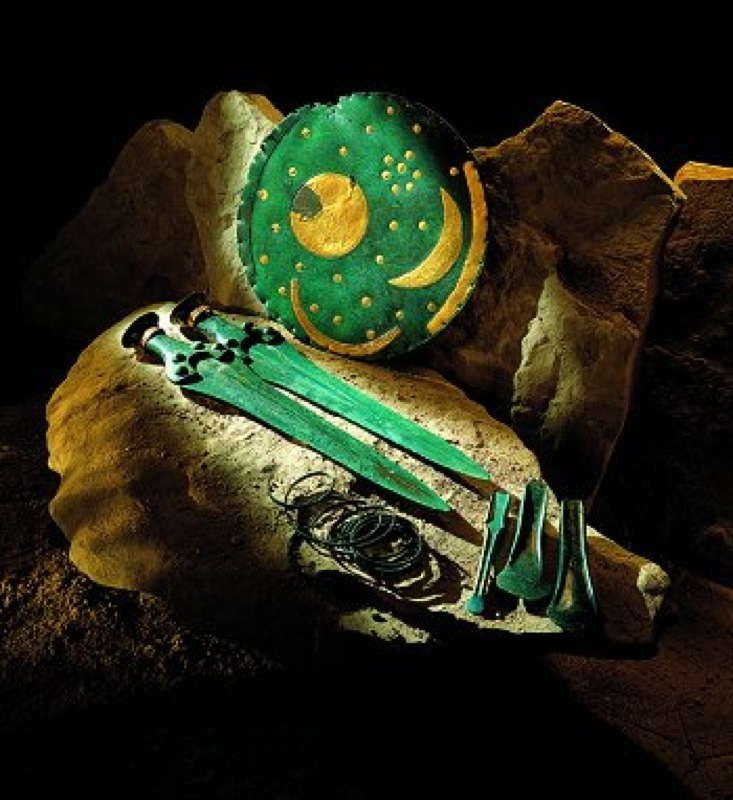
\includegraphics[width=0.618\textwidth]{pictures/babylonuhr.jpg}}
\title{Zahlen \& Rechnen}
\subtitle{I like $\mP$}
\author{}
\date{}
%\lowertitleback{
%\includegraphics[height=1.1cm]{/Users/jormawassmer/Pictures/logokoeniz.jpg}%
%\copyright Jorma Wassmer
%1. Auflage, Februar 2011
%}


\begin{document}
\maketitle

\tableofcontents
%\thispagestyle{empty}
\cleardoublepage
%\setcounter{page}{1}

\section{Mengenlehre}

\subsection{Historisches zur Mengenlehre}
\begin{wrapfigure}{r}{0.382\textwidth}
  \begin{center}
    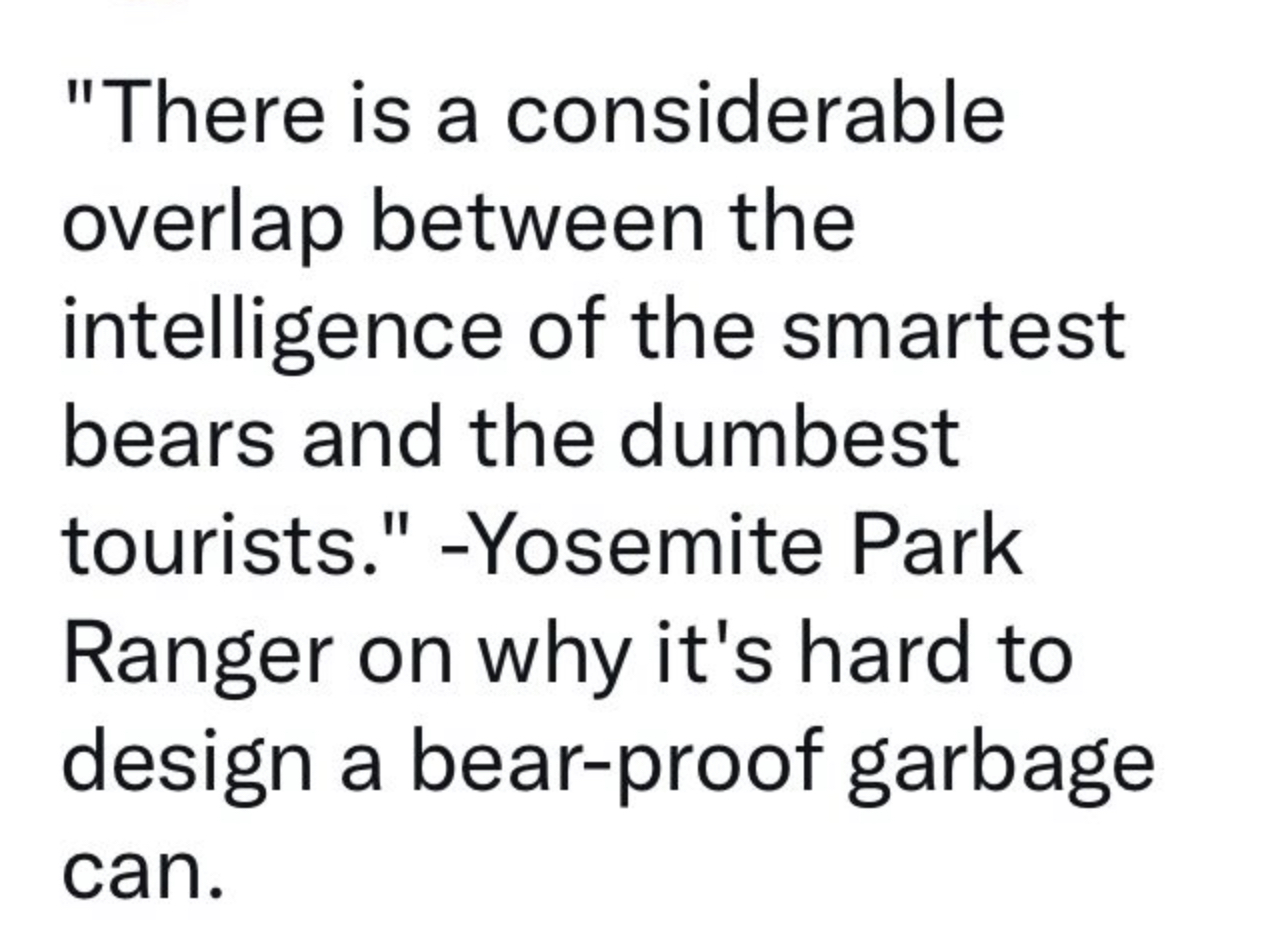
\includegraphics[width=0.382\textwidth]{pictures/schnittmenge.jpeg}
  \end{center}
\caption{Schnittmenge}
\end{wrapfigure}
Die Mengenlehre kann als Fundament der gesamten modernen Mathematik aufgefasst werden. Ihre Begriffe und Sprachelemente sind heute f\"ur die Formulierung mathematischer Probleme unentbehrlich geworden. Das Kapitel zu den Relationen und Funktionen wird zeigen, dass neue Begriffe mit den Mitteln, die die Mengenlehre zur Verf\"ugung stellt, sehr einfach definiert werden k\"onnen. Damit werden Sie einen tieferen Einblick in die Relationen- und Funktionenlehre erhalten.

Die axiomatische Mengenlehre ist ein relativ neuer mathematischer Gegenstand. Die wichtigsten Grundbegriffe gehen auf den deutschen Mathematiker \textsc{Georg Cantor} (1845--1918) zur\"uck. Seine erste mengentheoretische Arbeit erschien 1874. Erst sp\"ater aber erkannte man das Potenzial dieser Theorie. Nach einem Ausspruch von \textsc{David Hilbert}, einem bedeutenden deutschen Mathematiker (1862--1943), schuf \textsc{Cantor} mit seiner Mengenlehre
\begin{quote}
\glqq\dots einen der fruchtreichsten und kr\"aftigsten Wissenszweig der Mathematik, ein Paradies, aus dem uns niemand soll vertreiben k\"annen.\grqq
\end{quote}
Erst der Student der Mathematik wird sich mit Grenzen und Problemen der axiomatischen Mengenlehre auseinandersetzen d\"urfen; auf der Stufe Mittelschule besch\"aftigt man sich nur mit der \emph{naiven Mengenlehre}.

\subsection{Definition der Menge nach Cantor}
Unsere Sprache enth\"alt viele Ausdr\"ucke zur Bezeichnung von Mengen. Biologen verwenden Kategorien wie Ordnung, Familie, Gattung, um Pflanzen und Tiere, die gewisse Gemeinsamkeiten aufweisen, zusammenzufassen. Wirtschaftswissenschaftler unterteilen die Bev\"olkerung in verschiedene soziale Klassen. Psychologen befassen sich mit Batterien von Tests, \"Arzte mit Syndromen. Alle diese Ausdr\"ucke, wie Ansammlung, Kategorie, Klasse etc. haben eine gewisse gemeinsame Bedeutung. Die Mathematiker ihrerseits bevorzugen die Bezeichnung Menge.
\begin{cdef}[Menge]{}
Unter einer \emph{Menge}\index{Menge} versteht man jede Zusammenfassung von bestimmten wohlunterscheidbaren Objekten unserer Anschauung oder unseres Denkens zu einem Ganzen.
\end{cdef}

\begin{bem}
Es ist empfehlenswert, eine \emph{leere Menge} zu definieren. Die \emph{leere Menge}\index{Menge!leere} $\set{}=\emptyset$ ist die Menge, die kein Element enth\"alt.
\end{bem}

Es gibt zwei M\"aglichkeiten, eine Menge hinzuschreiben:
\begin{itemize}
\item die \emph{aufz\"ahlende} Form
\item die \emph{beschreibende} Form
\end{itemize}

\begin{cdef}[Element]{}
Die Objekte einer Menge nennt man \emph{Elemente} der Menge.
\end{cdef}

Es seien $a_1,a_2,a_3,\dots,a_n$ irgendwelche verschiedene Objekte. Diese Objekte lassen sich zu einer Menge $\D{G}$ zusammenfassen.
Elemente einer Menge werden in geschweifte Klammern gefasst. Man schreibt
$$\D{G}=\set{a_1,a_2,a_3,\dots,a_n}$$
\begin{bsp}
Die Menge der f\"unf traditionellen Sinne
$$\D{S}=\set{\text{sehen},\text{h\"aren},\text{riechen},\text{schmecken},\text{tasten}}$$
\end{bsp}
Mengen bezeichnet man \"ublicherweise mit Grossbuchstaben, Elemente mit Kleinbuchstaben. Zur Veranschaulichung benutzt man meist sogenannte \emph{Euler}- oder \emph{Venndiagramme}.

\begin{bem}
Um auszudr\"ucken, ob ein Element zu einer Menge $\D{G}$ geh\"art oder nicht, benutzt man die Symbole $\in$ (sprich \glqq ist Element von\grqq, oder kurz \glqq in\grqq) bzw. $\notin$ (sprich \glqq ist nicht Element von\grqq, oder kurz \glqq nicht in\grqq).
\end{bem}

\begin{figure}
\begin{center}
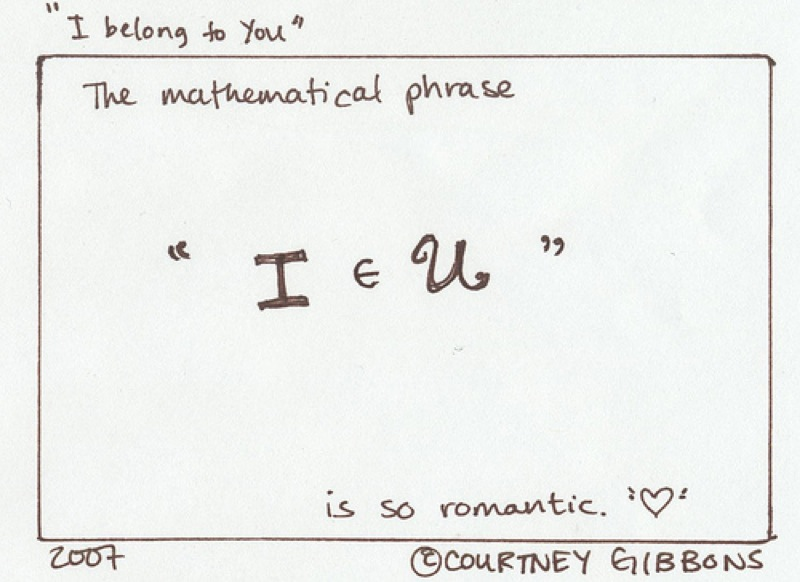
\includegraphics[width=0.45\textwidth]{pictures/belongsto}
\caption{\glqq ist Element von\grqq}
\end{center}
\end{figure}

\begin{ueb}[Menge oder nicht Menge, das ist hier die Frage]
Entscheide, ob es sich um eine Menge im mathematischen Sinn handelt. Begr\"unde deine Antwort.
\begin{enumeratea}
\item Alle Primzahlen kleiner als $20$.
\item Alle reichen Leute in der Schweiz.
\item Die Menge der Patienten eines Spitals.
\item Die Bremer Stadtmusikanten aus dem gleichnamigen M\"archen.
\end{enumeratea}
\end{ueb}

\begin{ueb}[explizit]
Schreibe die folgenden Mengen explizit auf. Benutze m\"aglicherweise Hilfsmittel (Atlas, google, \dots)
\begin{enumeratea}
\item Die Menge der Primzahlen kleiner als $30$
\item Die Menge der Staaten auf dem australischen Kontinent
\item Die Menge nat\"urlicher Satelliten der Erde
\end{enumeratea}
\end{ueb}

\begin{ueb}[in Worten]
Gib eine Beschreibung in Worten der folgenden Mengen an und f\"uge jeweils ein weiteres Element hinzu:
\begin{enumeratea}
\item $\set{a,e,i,o,\q}$
\item $\set{1972,1976,1980,\q}$
\item $\set{2,4,8,16,32,\q}$
\end{enumeratea}
\end{ueb}

\begin{ueb}[Mississippi]
Schreibe als Menge:
\begin{enumeratea}
\item die Buchstaben im Wort Mississippi
\item Grossbuchstaben mit einem Symmetriezentrum
\end{enumeratea}
\end{ueb}

\begin{ueb}[in or not in\dots]
Es sei $\D{A}$ die Menge der Konsonanten, $\D{B}$ die Menge der Vielfachen von $5$ und
$$\D{C}=\setm{x}{(x-5)(x+3)(x-2)=0}$$
Setze das richtige Zeichen ($\in$ oder $\notin$).
\begin{enumeratea}
\item $d\q\D{A}$
\item $5\q\D{C}$
\item $99\q\D{B}$
\end{enumeratea}
\end{ueb}

\begin{ueb}[aufz\"ahlen]
Es seien
\begin{align*}
\D{A}&=\set{1,3,5,7,9}\\
\D{B}&=\set{1,3,4,5,8}\\
\D{C}&=\set{1,3}\\
\D{D}&=\set{2,4,6}\\
\end{align*}
Schreibe folgende Mengen in aufz\"ahlender Form:
\begin{enumeratea}
\item $\setm{x}{x\in\D{A}, x\in\D{B}}$
\item $\setm{x}{x\in\D{A},x\in\D{B},x\notin\D{C}}$
\end{enumeratea}
\end{ueb}

\subsection{Historisches zu Zahlen}

\begin{wrapfigure}{r}{0.4\textwidth}
  \begin{center}
    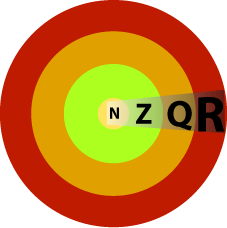
\includegraphics[width=0.3\textwidth]{pictures/zahlen}
  \end{center}
%\caption{A gull}
\end{wrapfigure}
Die Zahl und das Z\"ahlen haben im Leben der Menschen schon immer eine wichtige Rolle gespielt. Beim Z\"ahlen benutzte der Mensch die Finger, wie dies heute noch Naturv\"olker oder Kinder tun. Dies spiegelt sich auch in den alten Zahlenzeichen wieder. H\"aufig waren dies Striche oder Kerben. Alte Kulturv\"olker wie die Babylonier, \"Agypter oder R\"omer schufen bestimmte Symbole f\"ur die Zahlen $1,5,10,100,1000$ u.a. und bildeten damit durch Aneinanderreihen die \"ubrigen nat\"urlichen Zahlen.

In den ersten Jahrhunderten n.u.Z. gingen bei den Indern aus den Anfangsbuchstaben der Zahlw\"orter vermutlich jene Zeichen f\"ur die Zahlen $1$ bis $9$ hervor, aus denen sich sp\"ater unsere Ziffern $1,2,3,\dots,9$ entwickelten. Die Inder gaben diesen Ziffern einen Stellenwert und erfanden f\"ur eine leere Stelle ein besonderes Zeichen, die Null. Ein Stellenwertsystem und ein Zeichen f\"ur die Null hatten lange vor den Indern auch schon die Babylonier. Bei ihnen war $60$ die Grundzahl (Sexagesimalsystem). Nach und nach wurden die nat\"urlichen Zahlen erweitert. Die Inder kannten negative Zahlen f\"ur Schulden. Die Griechen entdeckten, das Wurzeln nicht immer als Bruch dargestellt werden k\"onnen.

Hier werden folgend \"ubliche Bezeichnungen und Notationen betreffend Zahlenmengen aufgef\"uhrt. Als Highlight soll die Existenz von irrationalen Zahlen anhand eines klassischen Beispiels illustriert werden.
\subsection{Bezeichnungen}
Die Menge der \emph{nat\"urlichen Zahlen} wird mit
$$\D{N}=\set{1,2,3,\dots}$$
abgek\"urzt.

Bei der Subtraktion von $3-3$ oder $4-5$ treten Schwierigkeiten auf, denn die Ergebnisse sind nicht mehr in den nat\"urlichen Zahlen enthalten. Deshalb werden den nat\"urlichen Zahlen bei Bedarf die Null
$$\D{N}_0=\set{0,1,2,3,\dots}$$
hinzugef\"ugt, oder, wie im zweiten Fall, auch die negativen Zahlen. Man erh\"alt so die Menge der \emph{ganzen Zahlen}
$$\D{Z}=\set{\dots,-3,-2,-1,0,1,2,3,\dots}.$$

Bei der Behandlung nichttrivialer Divisionen, wie etwa $2\div3$, entsteht ein weiteres Mal das Bed\"urfnis, das Zahlensystem zu erweitern. Zur Menge der ganzen Zahlen kommen die Br\"uche hinzu. Damit erh\"alt man die Menge der \emph{rationalen Zahlen}
$$\D{Q}=\setm{\frac{a}{b}}{a\in\D{Z}, b\in\D{N}}$$
In dieser Zahlenmenge k\"annen die vier Grundoperationen $+,-,\cdot,\div$ uneingeschr\"ankt durchgef\"uhrt werden; ausser die Division durch $0$. Man sagt:
\begin{quote}
$\D{Q}$ ist \emph{abgeschlossen} bez\"uglich allen vier Grundoperationen.
\end{quote}

\begin{bem}
Jede rationale Zahl l\"asst sich durch Division in einen Dezimalbruch verwandeln.
\end{bem}
Dabei treten zwei F\"alle auf:
\begin{itemize}
\item Nach endlich vielen Schritten tritt der Rest $0$ auf, d.h. der Dezimalbruch ist \emph{abbrechend}.
\item Der Rest $0$ tritt nie auf. Dann heisst der Dezimalbruch \emph{periodisch}.
\end{itemize}
\begin{bsps}
Die rationale Zahl
$$\frac{1}{8}=0.125$$
ist abbrechend. Dagegen ist
$$\frac{1}{7}=0.\overline{142857}$$
periodisch.
\end{bsps}
\begin{frage}
Kannst du obige Beispiele mit schriftlicher Division best\"atigen?
\end{frage}

\begin{bem}
Umgekehrt l\"asst sich jeder abbrechende oder periodische Dezimalbruch in einen gew\"ahnlichen Bruch verwandeln.
\end{bem}

\begin{bsp}
Bei den abbrechenden Dezimalbr\"uchen ist die Umwandlung einfach. Man bestimmt die Gr\"asse der letzten Nachkommastelle, schreibt als Bruch und k\"urzt gegebenenfalls:
$$0.25=\frac{25}{100}=\frac{1}{4}$$
Bei den periodischen hilft folgendes Vorgehen: Man definiert die gesuchte Zahl, die als Bruch dargestellt werden soll als $x$. Danach bestimmt man die L\"ange der Periode und den Wert des Vielfachen von $x$ mit der Periodenl\"ange. Anschliessend wird $x$ von diesem Produkt abgezogen und die entstandene Gleichung nach $x$ aufgel\"ast; voilˆ.
\begin{align}
0.\overline{12}&=x \notag\\ \notag
12.\overline{12}&=100x\\ \notag
12&=99x\\ \notag
\frac{12}{99}&=x\\ \notag
\frac{4}{33}&=x
\end{align}
\end{bsp}

\begin{bsp}
Es gibt aber offensichtlich Dezimalbr\"uche, die weder abbrechend noch periodisch sind.
$$0.1234567891011121314\dots$$
\end{bsp}

\begin{frage}
Kannst du einen nicht periodischen und nicht abbrechenden Dezimalbruch konstruieren, der nur Nullen und Einsen enth\"alt?
\end{frage}

Ein weiteres ber\"uhmtes Beispiel f\"ur eine nicht rationale Zahl ist die positive Zahl, deren Quadrat gleich $2$ ist, n\"amlich $\sqrt{2}$. Mit der folgenden Argumentation (indirekte Beweismethode)
\marginnote{
\qrcode{
https://www.youtube.com/watch?v=_ONbuGauF9I}
}
l\"asst sich dies leicht einsehen.

\begin{csatz}[Es gibt irrationale Zahlen]{satz:sqrt2irrational}
$\sqrt{2}$ ist nicht rational.
\end{csatz}

\begin{proof}[Beweis]
Wir wollen zeigen, dass $\sqrt{2}$ nicht rational ist. Dazu nehmen wir das Gegenteil der Behauptung an. K\"annen wir diese Gegenannahme auf einen Widerspruch f\"uhren, so muss die Gegenannahme falsch und somit die urspr\"ungliche Aussage richtig sein. (Tertium non datur)

Annahme $\sqrt{2}$ ist rational. Also gibt es eine Darstellung
$$\sqrt{2}=\frac{p}{q}$$
wobei $p,q\in\D{N}$ und der Bruch vollst\"andig gek\"urzt ist. Daraus folgt durch quadrieren und multiplizieren mit $q^2$
$$2q^2=p^2$$
Das bedeutet, das $p^2$, und damit $p$ eine gerade Zahl ist. Andererseits gilt
$$q^2=\frac{p^2}{2}=p\cdot\frac{p}{2}$$
Also ist $q^2$ und damit $q$ gerade. Widerspruch zur Annahme, dass $\frac{p}{q}$ vollst\"andig gek\"urzt sei. Dann der Bruch k\"annte sicher mit $2$ gek\"urzt werden, weil sowohl $p$ als auch $q$ gerade sind. Also ist $\sqrt{2}$ nicht rational.
\end{proof}

Auch von der Zahl $\pi$, dem Verh\"altnis von Umfang zum Durchmesser eines Kreises, weiss man, dass sie nicht rational sein kann. Der Beweis ist nicht so einfach und gelang \"ubrigens erst im $18.$ Jahrhundert. Diese und andere Tatsachen f\"uhren dazu, dass man eine umfassendere Zahlenmenge braucht, in der auch die oben genannten enthalten sind. F\"ur unsere Zwecke wird diese Menge ausreichend sein. Wir geben hier keine formale Definition, sondern beschreiben sie folgendermassen.

\begin{cdef}[Reelle Zahlen]{}
Die \emph{reellen Zahlen} entsprechen eindeutig s\"amtlichen Punkten der Zahlengeraden.
\end{cdef}
Demnach ist also auch jede rationale Zahl eine reelle. Wir unterscheiden noch durch
\begin{cdef}[Irrationael Zahlen]{}
Reelle Zahlen, die nicht rational sind, heissen \emph{irrational}.
\end{cdef}

\begin{frage}
Kannst du die Situation aller oben vorgestellten Zahlenmengen $\D{N}$, $\D{Z}$, $\D{Q}$, $\D{R}$ und $\D{I}$ in einem Eulerdiagramm skizzieren?
\end{frage}

\begin{ueb}[schriftlich dividieren]
Berechne mit Hilfe der schriftlichen Division den Wert von\\

(a) $\frac{1}{18}\q$ (b) $\frac{1}{15}\q$ (c) $\frac{3}{11}\q$ (d) $\frac{1}{17}$

\end{ueb}

\begin{ueb}[runter brechen]
Schreibe als rationale Zahl in Bruchform\\

(a) $0.1234\q$ (b) $0.\overline{3}\q$ (c) $0.\overline{14}\q$ (d) $2.\overline{9}$

\end{ueb}

\begin{ueb}[Zahlengerade]
Konstruiere auf einer Zahlengerade die Punkte\\

(a) $\sqrt{5}\q$ (b) $\frac{2}{3}\q$ (c) $-1\frac{1}{4}\q$ (d) $\sqrt{20}\q$ (e) $-\sqrt{3}\q$ (f) $0.\overline{7}$

\end{ueb}

\subsection{Kardinalit\"at einer Menge}
\begin{figure}
  \begin{center}
    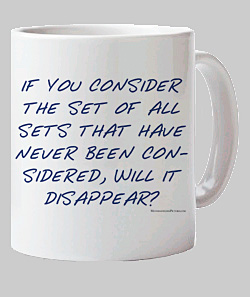
\includegraphics[width=0.382\textwidth]{pictures/sets}
  \end{center}
\caption{Is there a set of non considered sets?}
\end{figure}
Im t\"aglichen Leben verwendet man die nat\"urlichen Zahlen vor allem
\begin{itemize}
\item zum Nummerieren/Ordnen von Gegenst\"anden; die nat\"urlichen Zahlen dienen als \emph{Ordinalzahlen}.
\item als Anzahlen zur gr\"ossenm\"assigen Beschreibung von Mengen; als \emph{Kardinalzahlen}.
\end{itemize}

Wenn man Elemente einer Menge $\D{G}$ abz\"ahlt, so ist die letzte Zahl zugleich die Anzahl der Elemente dieser Menge.
\begin{cdef}[Kardinalität]{}
Die Anzahl der Elemente einer Menge $\D{G}$ heisst \emph{Kardinalit\"at} oder M\"achtigkeit von $\D{G}$. Man schreibt $\card(\D{G})$.
\end{cdef}
\begin{bsps}
F\"ur $\D{G}=\set{-2,-1,0,1,2}$ ist $\card(\D{G})=5$. Oder man hat $\card(\D{\emptyset})=0$.
\end{bsps}
\begin{bem}
Eine Menge kann auch eine unendliche Anzahl von Elementen enthalten; entsprechend spricht man von einer \emph{unendlichen} Menge.
\end{bem}

\subsection{Teilmenge}

\begin{cdef}[Teilmenge]{}
Ist
\marginnote{
\qrcode{
https://www.youtube.com/watch?v=FDNt0pE4jUA}
}
jedes Element einer Menge $\D{A}$ auch in einer Menge $\D{B}$ enthalten, so ist $\D{A}$ eine \emph{Teilmenge} von $\mB$. Man schreibt
$$\mA\subset\mB$$
\end{cdef}

\begin{bem}
Offensichtlich ist jede Menge Teilmenge von sich selbst.
\end{bem}

\begin{csatz}[Leere Menge]{}
Die
\marginnote{
\qrcode{
https://www.youtube.com/watch?v=SYxQy0rDctg}
}
leere Menge ist Teilmenge jeder Menge.
\end{csatz}

\begin{proof}[Beweis]
Gegenannahme: W\"are die leere Menge nicht Teilmenge jeder Menge, dann g\"abe es mindestens eine Menge, sagen wir $\mM$, welche die leere Menge nicht enthalten w\"urde. Dann m\"usste es aber nach Definition von Teilmenge ein Element $x$ in der leeren Menge geben, das nicht zu $\mM$ geh\"art. Widerspruch, denn somit w\"are die leere Menge ja nicht leer, weil sie dieses $x$ enthalten w\"urde. Also muss die leere Menge Teilmenge jeder Menge sein.
\end{proof}

Haben zwei Mengen $\mA$ und $\mB$ die gleichen Elemente, so schreibt man $\mA=\mB$.

\subsection{Operationen}
\marginnote{
\qrcode{
https://www.youtube.com/watch?v=nvYwG5cJGWA}
}
\subsubsection{Durchschnittsmenge}
\begin{cdef}[Schnitt]{}
Die \emph{Durchschnittsmenge} zweier Mengen $\mA$ und $\mB$ besteht aus s\"amtlichen Elementen, die sowohl zu $\mA$ als auch zu $\mB$ geh\"aren. In mathematischer Schreibweise
$$\mA\cap\mB=\setm{x}{x\in\mA\text{ und }x\in\mB}$$
\end{cdef}

\def\firstcircle{(0,0) circle (1.5cm)}
\def\secondcircle{(0:2cm) circle (1.5cm)}
\def\grundmenge{(-3,-2) rectangle (3,2)}

\colorlet{circle edge}{blue!50}
\colorlet{circle area}{blue!20}

\colorlet{rectangle edge}{blue!50}
\colorlet{rectangle area}{blue!20}

\tikzset{filled/.style={fill=circle area, draw=circle edge, thick},
    outline/.style={draw=circle edge, thick}}

% Set A and B
\begin{center}
\begin{tikzpicture}
    \begin{scope}
        \clip \firstcircle;
        \fill[filled] \secondcircle;
    \end{scope}
    \draw[outline] \firstcircle node {$\mA$};
    \draw[outline] \secondcircle node {$\mB$};
    \node[anchor=south] at (current bounding box.north) {$\mA \cap \mB$};
\end{tikzpicture}
\end{center}

\begin{bsp}
Ist $\mA=\set{1,2}$ und $\mB=\set{2,3}$, dann gilt
$$\mA\cap\mB=\set{2}$$
\end{bsp}
\begin{cdef}[disjunkt]{}
Zwei Mengen heissen \emph{disjunkt}, wenn sie keine gemeinsamen Elemente haben, d.~h.
$$\mA\cap\mB=\emptyset$$
\end{cdef}

\pagebreak

\subsubsection{Vereinigungsmenge}
\begin{cdef}[Vereinigung]{}
Die \emph{Vereinigunsmenge} zweier Mengen $\mA$ und $\mB$ besteht aus s\"amtlichen Elementen, die zu $\mA$ oder $\mB$ geh\"aren. Man schreibt
$$\mA\cup\mB=\setm{x}{x\in\mA\text{ oder }x\in\mB}$$
\end{cdef}

\begin{center}
% Set A or B
\begin{tikzpicture}
    \draw[filled] \firstcircle node {$\mA$}
                  \secondcircle node {$\mB$};
    \node[anchor=south] at (current bounding box.north) {$\mA \cup \mB$};
\end{tikzpicture}
\end{center}

\begin{bsp}
F\"ur $\mA$ und $\mB$ wie im obigen Beispiel gilt
$$\mA\cup\mB=\set{1,2,3}$$
\end{bsp}

\subsubsection{Differenzmenge}
\begin{cdef}[Differenz]{}
Die \emph{Differenzmenge} von $\mA$ mit $\mB$ besteht aus s\"amtlichen Elementen, die zu $\mA$, aber nicht zu $\mB$ geh\"aren. Man schreibt
$$\mA\setminus\mB=\setm{x}{x\in\mA\text{ und }x\notin\mB}$$
\end{cdef}

\begin{center}
% Set A but not B
\begin{tikzpicture}
    \begin{scope}
        \clip \firstcircle;
        \draw[filled, even odd rule] \firstcircle node {$\mA$}
                                     \secondcircle;
    \end{scope}
    \draw[outline] \firstcircle
                   \secondcircle node {$\mB$};
    \node[anchor=south] at (current bounding box.north) {$\mA\setminus \mB$};
\end{tikzpicture}
\end{center}

\begin{bsp}
Mit $\mA$ und $\mB$ wie oben gilt
$$\mA\setminus\mB=\set{1}$$
\end{bsp}

\subsubsection{Komplement\"armenge}
\begin{cdef}[Komplement]{}
Es sei $\mA\subset\mG$. Das \emph{Komplement} von $\mA$ bez\"uglich der Grundmenge $\mG$ besteht aus s\"amtlichen Elementen von $\mG$, die nicht zu $\mA$ geh\"aren. Man schreibt
$$\overline{\mA}=\setm{x}{x\in\mG\text{ und }x\notin\mA}$$
\end{cdef}

\begin{center}
\begin{tikzpicture}
    \begin{scope}
        \clip \grundmenge;
        \draw[filled, even odd rule] \grundmenge node[anchor=north east] {$\overline{\mA}$}
                                     \firstcircle;
    \end{scope}
    \draw[outline] \firstcircle node {$\mA$};
    \node[anchor=south] at (current bounding box.north) {$\mG$};
\end{tikzpicture}
\end{center}

\begin{bsp}
Ist $\mG=\set{1,2,3}$ und $\mA$ wie oben, dann gilt
$$\overline{\mA}=\set{3}$$
\end{bsp}

\begin{ueb}[Kapitel]
Es seien
\begin{align}
\D{A}&=\set{k,a,p,i,t,e,l}\notag\\
\D{B}&=\set{t,e,i,l}\notag\\
\D{C}&=\set{k,a,p}\notag\\
\D{D}&=\set{}\notag\\
\D{E}&=\set{e,i,s}\notag
\end{align}
Welche der folgenden Aussagen sind richtig?\\

(a) $\D{E}\subset\D{A}\q$ (b) $\D{A}\subset\D{B}\q$ (c) $\D{B}\subset\D{A}\q$ (d) $\D{D}\subset\D{C}\q$ (e) $\D{C}\subset\D{A}\q$ (f) $\D{E}\subset\D{D}$

\end{ueb}

\begin{ueb}[richtig oder falsch]
Welche der folgenden Aussagen sind richtig?\\[2ex]
\hspace*{2.7ex}
\begin{minipage}{0.4\textwidth}
\begin{enumeratea}
\item $0\notin\emptyset$
\item $0\subset\set{0,1,2}$
\item $\emptyset\in\set{1,2,3}$
\item $\emptyset\subset{0}$
\item $\emptyset=\setm{x}{x\neq x}$
\end{enumeratea}
\end{minipage}
\begin{minipage}{0.3\textwidth}
\begin{enumeratea}\addtocounter{enumi}{5}
\item $\set{1,2}\not\subset\set{2,1}$
\item $\emptyset\in\set{0}$
\item $\set{a}\in\set{a,\set{a}}$
\item $\emptyset\subset\set{\emptyset,\set{a}}$
\item $\emptyset\in\set{\emptyset,\set{a}}$
\end{enumeratea}
\end{minipage}
\end{ueb}

\begin{cdef}[Potenzmenge]{}
Die Menge aller Teilmengen einer Menge $\mA$ heisst \emph{Potenzmenge} von $\mA$.
$$\mathcal{P}(\mA)=\setm{\mB}{\mB\subset\mA}.$$
\end{cdef}

\begin{bsp}
Die Potenzmenge von $\mA=\set{1,2}$ ist
$$\mathcal{P}(\mA)=\set{\set{},\set{1},\set{2},\set{1,2}}$$
\end{bsp}

\begin{ueb}[Potenzmenge]
Bestimme die Potenzmenge $\mathcal{P}(\D{A})$ von
$$\D{A}=\set{a,b,c}$$
\end{ueb}

\begin{ueb}[Kardinalit\"at der Potenzmenge]
Wie viele Elemente hat die Potenzmenge einer Menge $\D{A}$ mit $\card(\D{A})=n$?
\end{ueb}

\begin{ueb}[Zahlen]
Es sei die Grundmenge
$$\D{G}=\set{1,2,3,4,\dots,19,20}$$
sowie Teilmengen von $\mG$
\begin{align*}
\D{A}&=\setm{x\in\D{G}}{x\text{ ist Viererzahl}}\\
\D{B}&=\set{8,9,10,11,12,13}\\
\D{C}&=\setm{x\in\D{G}}{x\text{ ist ungerade}}
\end{align*}

Ermittle

(a) $\D{A}\cap\D{B}\q$ (b) $\D{A}\cap\D{C}\q$ (c) $\overline{\D{C}\cup\D{B}}\q$ (d) $\overline{\D{C}}\setminus\D{A}$

\end{ueb}

\begin{ueb}[R\"uckschluss]
Es seien $\D{G}=\set{1,2,3,4}$ und $\D{A}=\set{1,2}$. Bestimme die Menge $\D{B}$ so, dass $\D{B}\cap\D{A}=\set{1}$ und $\D{B}\cup\D{A}=\D{G}$.
\end{ueb}

\begin{ueb}[Zahlenmengen]
Ermittle\\

(a) $\D{R}\cap\D{Q}\q$ (b) $(\D{N}\cap\D{Z})\cup\D{Q}\q$ (c) $\D{R}\cup(\D{Z}\cap\D{Q})$

\end{ueb}

\begin{ueb}[Ausschluss]
Von $45$ Sch\"ulerinnen nehmen $26$ an einer Arbeitsgemeinschaft f\"ur Physik, $14$ an einer Arbeitsgemeinschaft f\"ur Chemie teil. Wie viele Sch\"ulerinnen nehmen mindestens an keiner der beiden Arbeitsgemeinschaften teil, wie viele h\"achstens?
\end{ueb}

\begin{ueb}[etwas Logik]
Betrachte folgende Mengen: Grundmenge
$$\D{G}=\setm{x}{x\text{ ist Klubmitglied}}$$
\begin{align*}
\D{A}&=\setm{x}{x\text{ tr\"agt eine Krawatte}}\\
\D{B}&=\setm{x}{x\text{ hat seinen Arbeitsplatz in Basel}}\\
\D{C}&=\setm{x}{x\text{ hat braune Augen}}\\
\D{D}&=\setm{x}{x\text{ ist \"alter als 20 Jahre}}
\end{align*}
\begin{enumeratea}
\item Übersetze $\D{A}\cap\overline{\D{D}}=\emptyset$, $\D{B}\cap\D{C}=\D{B}$, $\D{A}\cup\D{C}=\D{G}$ jeweils in einen Satz unserer Umgangssprache.
\item Übersetze die folgenden S\"atze in die Mengensprache:\\
Es gibt keine Klubmitglieder mit braunen Augen, die \"alter als 20 Jahre sind.\\
Alle Klubmitglieder, die eine Krawatte tragen, arbeiten in Basel.
\end{enumeratea}
\end{ueb}

\begin{ueb}[noch etwas mehr Logik]
Es seien $\D{A}$ und $\D{B}$ zwei Mengen mit $\D{A}\cup\D{B}=\D{B}$. Welche der folgenden Aussagen ist immer richtig?\\
$\D{A}\subset\D{B}$, $\D{A}\cap\D{B}=\D{B}$, $\D{B}\subset\D{A}$, $\D{A}=\D{B}$, $\D{A}=\emptyset$.
\end{ueb}

\begin{ueb}[Planung]
Von den 26 Sch\"ulerinnen einer Klasse spielen 17 Fussball, 12 Schach und 9 Tennis. Eine Sch\"ulerin spielt gar nichts, 2 spielen alles, 3 spielen Schach und Tennis und 7 Schach und Fussball. Wie viele spielen nur Fussball und wie viele nur Tennis?
\end{ueb}

\cleardoublepage

\section{Polynome und Brüche}

\subsection{Grundlagen}

Los geht's!
\begin{itemize}
\item Algebra 1, Deller/Gebauer/Zinn, p.33--55
\item Algebra 1, Deller/Gebauer/Zinn, p.95--108
\item Theorie und Arbeitsblätter
\end{itemize}
Polynome und Bruchterme bilden die Bausteine vieler Berechnungen und mathematischer Theorien.
\begin{wrapfigure}{r}{0.4\textwidth}
  \begin{center}
    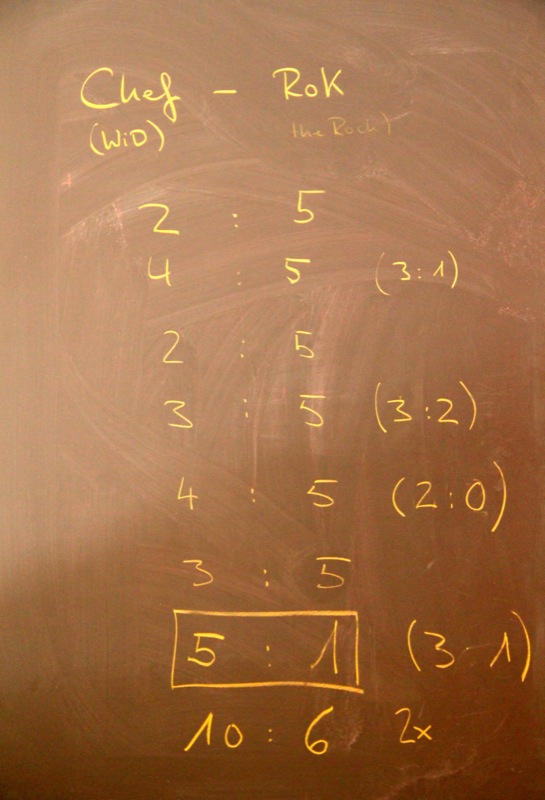
\includegraphics[width=0.22\textwidth]{pictures/rokwidboard}
  \end{center}
%\caption{A gull}
\end{wrapfigure}
Deshalb gehört die Fähigkeit, mit Polynomen sicher umgehen zu können, zu den grundlegendsten Voraussetzungen um Technik und Anwendungen der Neuzeit verstehen zu können; und nicht zuletzt um eine erfolgreiche gymnasiale Laufbahn einzuschlagen. Ein gutes Verständnis von Polynomen ist auch für den Umgang mit Bruchtermen wesentlich.

\subsection{Polynome}
Ihr solltet nach diesem Auftrag

\begin{itemize}
\item wissen, was Polynome und insbesondere Monome und Binome sind.
\item die binomischen Formeln beherrschen.
\item Polynome in ihrer Normalform darstellen können.
\item das Pascal'sche Dreieck zur Berechnung von Binomen nutzen.
\item Polynome faktorisieren können.
\item verstehen, was der Fundamentalsatz der Algebra aussagt.
\item den Divisionsalgorithmus auch auf Polynome anwenden können.
\end{itemize}

\subsection{Bruchterme und Polynome}
Es wird vorausgesetzt, dass ihr mit Zahlen und einzelnen Variablen Bruchrechnen könnt. Nun kommt neu dazu:

\begin{itemize}
\item Bruchterme beliebig zu erweitern und voll\-st\"an\-dig zu kürzen.
\item mit Bruchtermen jeglicher Art zu operieren.
\item mit Doppelbr\"uchen umzugehen.
\item \"Aquivalenzumformungen bei Bruchtermen zu erkennen.
\end{itemize}

Es sollten die unten aufgef\"uhrten Aufgaben erledigt werden. Daf\"ur stehen dir ca.~20 Lektionen mit allf\"alliger Hausarbeit zur Verf\"ugung. Zusatzaufgaben sind mit einem $^\star$ gekennzeichnet.
\subsubsection{Auftrag Polynome (p. 32--54)}
3, 7, 11, 29, 37(Addition \&\ Subtraktion); 45, 59, 81, 91 (Multiplikation); 115, 125, 127 (einfache Division); 139, 141 , 145 ,149, 153 (Binomische Formeln); 167, 193 (Pascal'sches Dreieck); 195, 197, 199, 205, 209 (Ausklammern); 239,241, 245, 247, 253, 259, 267 (Faktorzerlegung); 285, 287 (Polynomdivision).

\subsubsection{Auftrag Bruchterme (p. 94--108)}
13, 15, 19, 21, 23, 33, 35, 43, 49, 51 (K\"urzen und Erweitern); 57, 59, 61, 67, 73, 79 (Addition und Subtraktion); 91, 93, 95, 101, 107, 110, 121, 129, 135 (Multiplikation und Division); 143, 145, 149, 151 (Doppelbr\"uche);

\clearpage

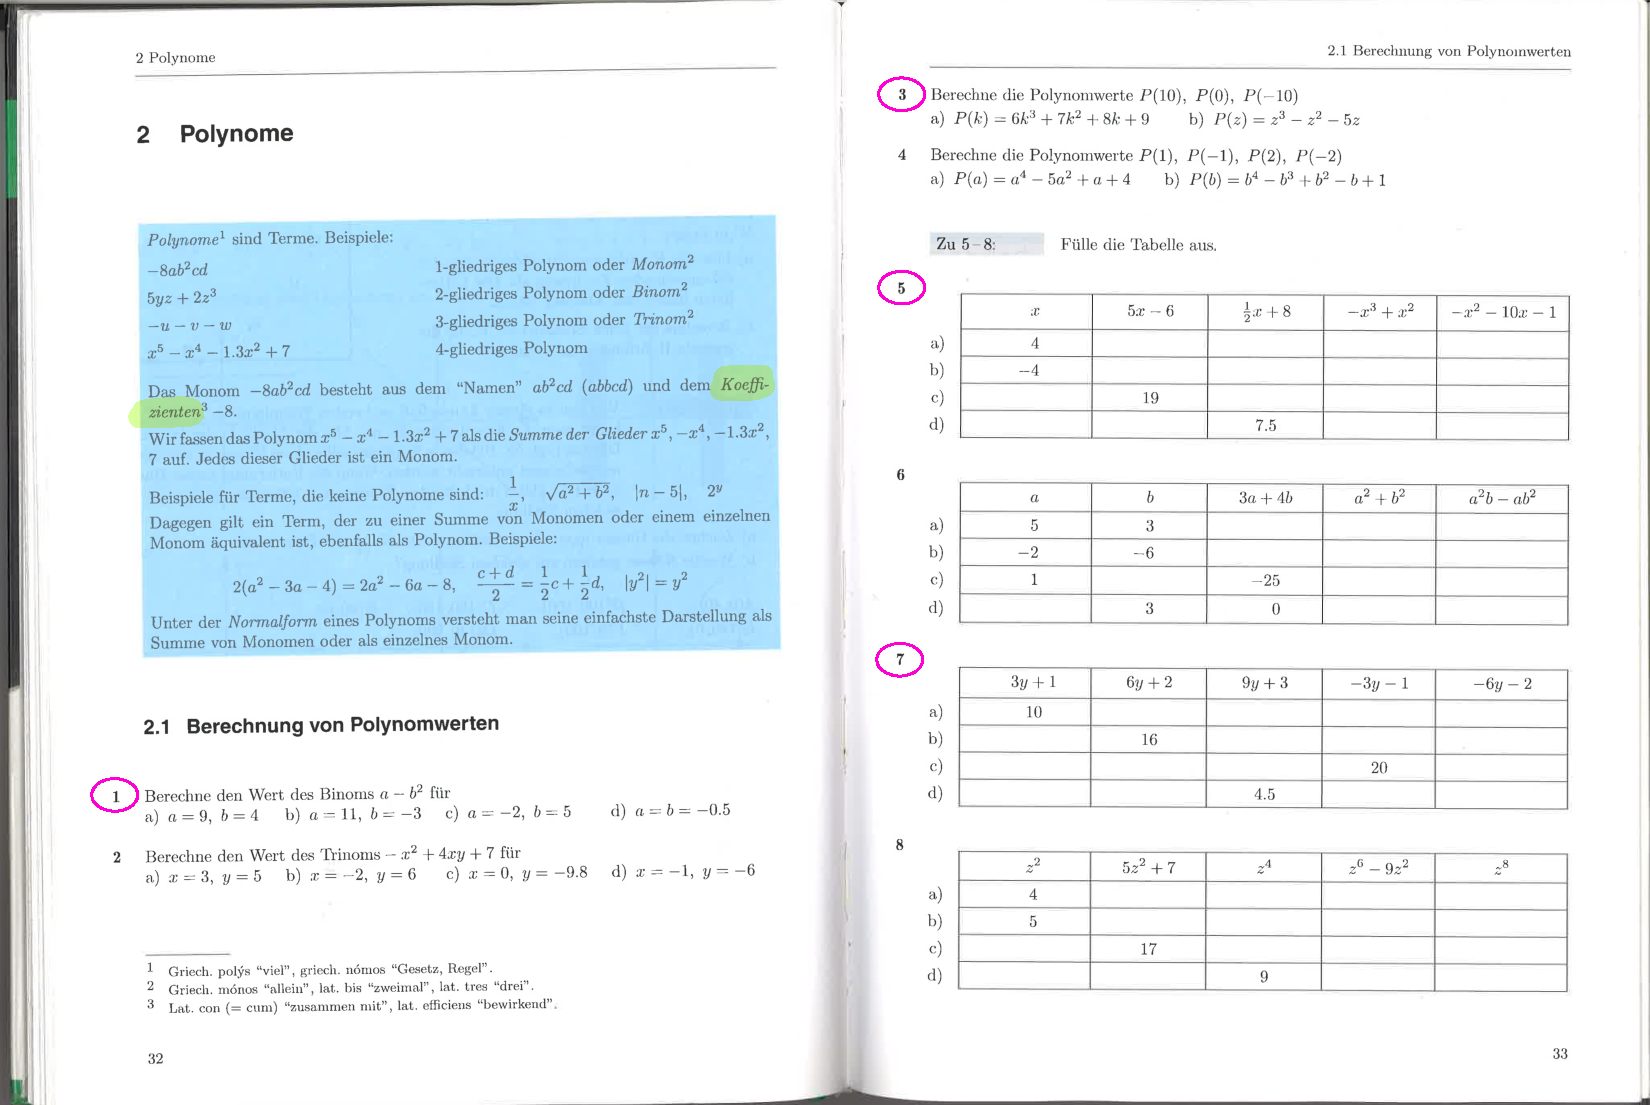
\includepdf[pages=1-2,pagecommand=\subsection{Aufgaben zu Polynome},scale=0.7,nup=1x2]{pictures/Algebra 1 Kapitel 2 Polynome Aufgaben.pdf}
\includepdf[pages=3-12,width=0.8\textheight,nup=1x2]{pictures/Algebra 1 Kapitel 2 Polynome Aufgaben.pdf}

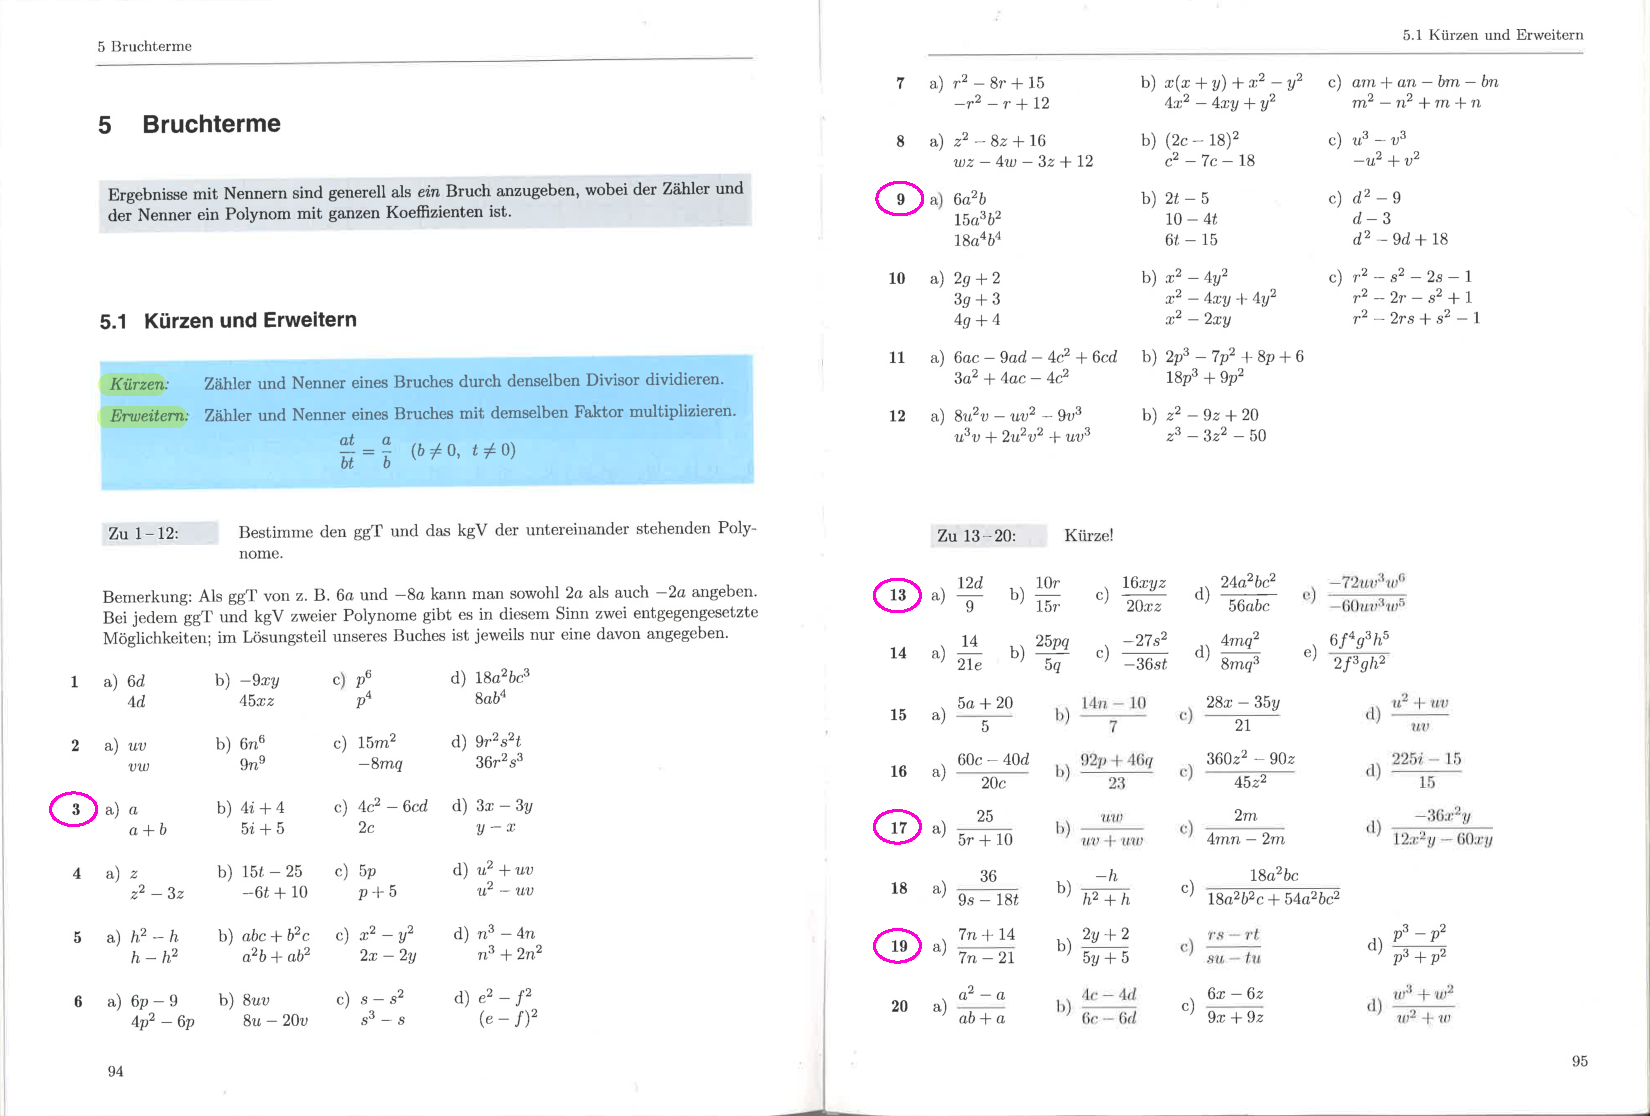
\includepdf[pages=1,pagecommand=\subsection{Aufgaben zu Brüche},scale=0.7,angle=90]{pictures/Algebra 1 Kapitel 5 Bruchterme Aufgaben.pdf}
\includepdf[pages=2-11,width=0.8\textheight,nup=1x2]{pictures/Algebra 1 Kapitel 5 Bruchterme Aufgaben.pdf}

\cleardoublepage

\section{Zehnerpotenzen}

\begin{wrapfigure}{r}{0.318\textwidth}
  \begin{center}
    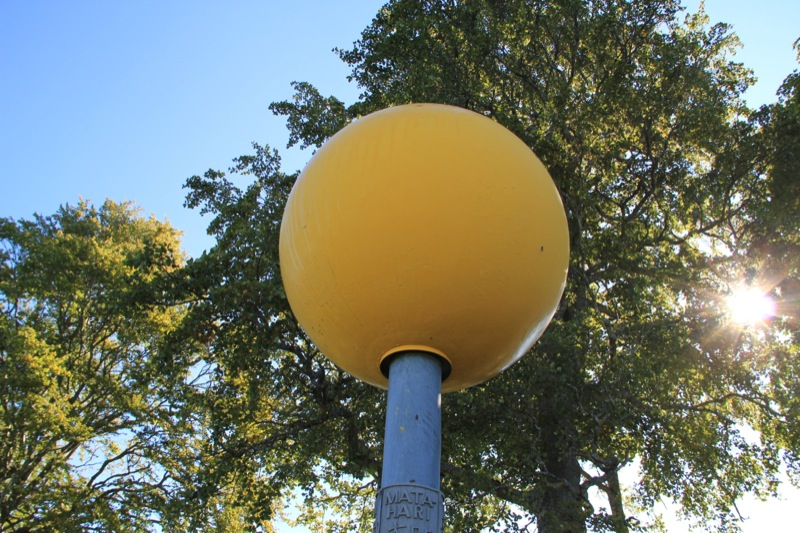
\includegraphics[width=0.318\textwidth]{pictures/sonne}
  \end{center}
%\caption{A gull}
\end{wrapfigure}
H\"aufig treten in allt\"aglichen oder wissenschaftlichen Kontexten, zum Beispiel in Physik, Biologie oder Chemie, grosse oder kleine Zahlen auf. Potenzen k\"onnen dazu verwendet werden um sehr grosse oder sehr kleine Zahlen kurz und \"ubersichtlich zu notieren. Zwei wichtige Beispiele f\"ur solche Zahlen sind folgend aufgef\"uhrt.

\begin{itemize}
\item Abstand Erde-Sonne, eine astronomische Einheit (1 AE)
$$\unit[150'000'000]{km}$$
\item Durchmesser eines Atoms, ein \AA ngstr\"om (1 \AA)
$$\unit[0.000\,000\,000\,1]{m}$$
\end{itemize}

\subsection{Der Potenzbegriff für natürliche Exponenten}
\begin{cdef}[Potenz, Basis und Exponent]{}
Der Term
$$a^b$$
heisst \emph{Potenz}. $a$ nennt man \emph{Basis}, $b$ heisst \emph{Exponent}.
\end{cdef}

\begin{cdef}[Potenz]
F\"ur $a\in\mR$ und $n\in\mN$ soll gelten:
$$a^1=a\q\text{ und }\q a^n=\underbrace{a\cdot a\cdot a\cdot\dots\cdot a}_{\text{n Faktoren}}\text{ f\"ur }n\geq2$$
\end{cdef}

\begin{bsps}
\ \\[-2ex]
\begin{itemize}
\item $2^3=2\cdot2\cdot2=8$
\item $\left(\frac{1}{3}\right)^2=\frac{1}{3}\cdot\frac{1}{3}=\frac{1}{9}$
\item $\pi^4\approx 3^4=81$
\end{itemize}
\end{bsps}

\subsection{Zehnerpotenzen}
Nach Definition gilt also zum Beispiel
$$10^1=10\q10^2=100\q10^3=1000$$
was leicht berechnet werden kann. Die obige Liste weist auch ein System auf: Erh\"oht man n\"amlich den Exponenten einer Zehnerpotenz um $1$, so muss man einfach die entsprechende Zahl mit $10$ multiplizieren. Wenden wir dieses Prinzip r\"uckw\"arts an, so k\"onnen wir Bedeutungen f\"ur die bislang sinnlosen Ausdr\"ucke
$$10^0\q10^{-1}\q10^{-2}\q\text{etc.}$$
festlegen. N\"amlich
$$10^0=1\q10^{-1}=0.1\q10^{-2}=0.01\q\dots$$

Lernen Sie zu den jeweiligen Zehnerpotenzen auch die entsprechenden Pr\"afixe und Ab\-k\"ur\-zungen, vielleicht mit Tabelle \ref{tab:zehnerpotenzen} auf Seite \pageref{tab:zehnerpotenzen}. Sie geh\"oren einer umfassenden Allgemeinbildung, da sie uns im Alltag begegnen. Damit l\"asst sich leicht erkl\"aren, wie viel ein Milliliter ist, was man unter einer Dekade versteht, wie viele Bytes ein Terabyte sind oder was unter den Begriff Mikrokosmos f\"allt. Auch eine namhafte Firma scheut sich nicht davor, ihr Flaggschiff i*** Nano zu nennen, um zu suggerieren, dass \dots.

\begin{table}
\begin{center}
\scalebox{0.9}{
  \begin{tabular}[ht]{lrlll}
    \rule[-3mm]{0mm}{24pt}
    $10^{12}\qq$ & $1\,000\,000\,000\,000$ & $\qq\qq\qq1$ Billion & \hspace*{1cm}Tera- & T\\
    \rule[-3mm]{0mm}{24pt}
    $10^{11}\qq$ & $100\,000\,000\,000$ &  &  & \\
    \rule[-3mm]{0mm}{24pt}
    $10^{10}\qq$ & $10\,000\,000\,000$ &  &  & \\
    \rule[-3mm]{0mm}{24pt}
    $10^{9}\qq$ & $1\,000\,000\,000$ & $\qq\qq\qq1$ Milliarde & \hspace*{1cm}Giga- & G\\
    \rule[-3mm]{0mm}{24pt}
    $10^{8}\qq$ & $100\,000\,000$ &  &  & \\
    \rule[-3mm]{0mm}{24pt}
    $10^{7}\qq$ & $10\,000\,000$ &  &  & \\
    \rule[-3mm]{0mm}{24pt}
    $10^{6}\qq$ & $1\,000\,000$ & $\qq\qq\qq1$ Million & \hspace*{1cm}Mega- & M\\
    \rule[-3mm]{0mm}{24pt}
    $10^{5}\qq$ & $100\,000$ &  &  & \\
    \rule[-3mm]{0mm}{24pt}
    $10^{4}\qq$ & $10\,000$ &  &  & \\
    \rule[-3mm]{0mm}{24pt}
    $10^{3}\qq$ & $1\,000$ & $\qq\qq\qq1$ Tausend & \hspace*{1cm}Kilo- & k\\
    \rule[-3mm]{0mm}{24pt}
    $10^{2}\qq$ & $100$ &  & \hspace*{1cm}Hekto- & h\\
    \rule[-3mm]{0mm}{24pt}
    $10^{1}\qq$ & $10$ &  & \hspace*{1cm}Deka- & d\\
    \rule[-3mm]{0mm}{24pt}
    $10^{0}\qq$ & $1$ &  &  & \\
    \rule[-3mm]{0mm}{24pt}
    $10^{-1}\qq$ & $0.1$ &  & \hspace*{1cm}Dezi- & d\\
    \rule[-3mm]{0mm}{24pt}
    $10^{-2}\qq$ & $0.01$ &  & \hspace*{1cm}Centi- & c\\
    \rule[-3mm]{0mm}{24pt}
    $10^{-3}\qq$ & $0.001$ & $\qq\qq\qq1$ Tausendstel & \hspace*{1cm}Milli- & m\\
    \rule[-3mm]{0mm}{24pt}
    $10^{-4}\qq$ & $0.000\,1$ &  &  & \\
    \rule[-3mm]{0mm}{24pt}
    $10^{-5}\qq$ & $0.000\,01$ &  &  & \\
    \rule[-3mm]{0mm}{24pt}
    $10^{-6}\qq$ & $0.000\,001$ & $\qq\qq\qq1$ Millionstel & \hspace*{1cm}Mikro- & $\mu$\\
    \rule[-3mm]{0mm}{24pt}
    $10^{-7}\qq$ & $0.000\,000\,1$ &  &  & \\
    \rule[-3mm]{0mm}{24pt}
    $10^{-8}\qq$ & $0.000\,000\,01$ &  &  & \\
    \rule[-3mm]{0mm}{24pt}
    $10^{-9}\qq$ & $0.000\,000\,001$ & $\qq\qq\qq1$ Milliardstel & \hspace*{1cm}Nano- & n\\
    \rule[-3mm]{0mm}{24pt}
    $10^{-10}\qq$ & $0.000\,000\,000\,1$ &  &  & \\
    \rule[-3mm]{0mm}{24pt}
    $10^{-11}\qq$ & $0.000\,000\,000\,01$ &  &  & \\
    \rule[-3mm]{0mm}{24pt}
    $10^{-12}\qq$ & $0.000\,000\,000\,001$ & $\qq\qq\qq1$ Billionstel & \hspace*{1cm}Piko & p\\
  \end{tabular}
  }
    \end{center}
    \caption{Zehnerpotenzen: Namen und Abk\"urzungen}\label{tab:zehnerpotenzen}
 \end{table}

\subsection{Wissenschaftliche Darstellung}
Wir kommen auf unsere Motivation zu Beginn des Kapitels zur\"uck; der schlanken Darstellung grosser und kleiner Zahlen. Bei der sogenannten \emph{wissenschaftlichen Darstellung} von Zahlen schreibt man die Zahl als Dezimalbruch mit Einer und Zehnerpotenzen.
\begin{bsps}
\ \\[-2ex]
\begin{itemize}
\item Abstand Erde-Sonne, eine astronomische Einheit (1 AE)
$$\unit[150'000'000]{km}=\unit[1.5\cdot10^8]{km}$$
\item Durchmesser eines Atoms, ein \AA ngstr\"om (1 \AA)
$$\unit[0.000\,000\,000\,1]{m}=\unit[1\cdot10^{-10}]{m}$$
\item $$92'300=9.23\cdot10^4$$
\item $$0.0032=3.2\cdot10^{-3}$$
\end{itemize}
\end{bsps}

\begin{bem}
Man findet leicht eine Merkregel, um den jeweiligen Wert des Exponenten zur Basis $10$ zu bestimmen.
\end{bem}

\begin{ueb}[expand]
  Schreibe die Zahlen aus:
  \\[2.5ex]\hspace*{2.7ex}
  \begin{minipage}{0.4\textwidth}
    \begin{enumeratea}
      \item $2.52\cdot10^{5}$
      \item $6.52\cdot10^{7}$
      \item $5.555\cdot10^{12}$
      \item $4.15\cdot10^{9}$\\[1ex]
    \end{enumeratea}
  \end{minipage}
  \begin{minipage}{0.23\textwidth}
    \begin{enumeratea}\addtocounter{enumi}{4}
      \item $4.31\cdot10^{9}$
      \item $3.11\cdot10^{3}$
      \item $1.23\cdot10^{6}$
      \item $6.22\cdot10^{4}$\\[1ex]
    \end{enumeratea}
  \end{minipage}
\end{ueb}

\begin{ueb}[factor]
  Schreibe in wissenschaftlicher Darstellung:
  \\[2.5ex]\hspace*{2.7ex}
  \begin{minipage}{0.4\textwidth}
    \begin{enumeratea}
      \item $99'000'000$
      \item $4'180'000'000$
      \item $48'500'000$
      \item $0.000\,008\,21$
      \item $92'400$
      \item $0.000\,016$\\[1ex]
    \end{enumeratea}
  \end{minipage}
  \begin{minipage}{0.4\textwidth}
    \begin{enumeratea}\addtocounter{enumi}{6}
      \item $19'300$
      \item $2'340$
      \item $1'350'000$
      \item $0.000\,000\,000\,101$
      \item $822'000'000$
      \item $0.000\,000\,077$\\[1ex]
    \end{enumeratea}
  \end{minipage}
\end{ueb}


\begin{ueb}[sci]
  Schreibe in wissenschaftlicher Darstellung:
  \\[2.5ex]\hspace*{2.7ex}
  \begin{minipage}{0.4\textwidth}
    \begin{enumeratea}
      \item $0.000\,015$
      \item $0.000\,008\,1$
      \item $0.654$
      \item $0.000\,000\,074$\\[1ex]
    \end{enumeratea}
  \end{minipage}
  \begin{minipage}{0.4\textwidth}
    \begin{enumeratea}\addtocounter{enumi}{4}
      \item $0.000\,000\,25$
      \item $0.000\,005\,15$
      \item $0.000\,000\,061\,5$
      \item $0.000\,000\,000\,077$\\[1ex]
    \end{enumeratea}
  \end{minipage}
\end{ueb}

\begin{ueb}[float]
  Schreibe die Zahlen aus:
  \\[2.5ex]\hspace*{2.7ex}
  \begin{minipage}{0.4\textwidth}
    \begin{enumeratea}
      \item $1.25\cdot10^{-5}$
      \item $7.22\cdot10^{-7}$
      \item $3.33\cdot10^{-12}$
      \item $4.15\cdot10^{-4}$
\\[1ex]
    \end{enumeratea}
  \end{minipage}
  \begin{minipage}{0.23\textwidth}
    \begin{enumeratea}\addtocounter{enumi}{4}
      \item $2.31\cdot10^{-9}$
      \item $2.75\cdot10^{-5}$
      \item $5.05\cdot10^{-6}$
      \item $6.02\cdot10^{-8}$\\[1ex]
    \end{enumeratea}
  \end{minipage}
\end{ueb}

\subsection{Rechenregeln f\"ur Potenzen}
Insbesondere beim Rechnen mit Variablen aber auch f\"urs Kopfrechnen k\"onnen folgende Regeln zu Hilfe genommen werden.

Wir erinnern uns an die Definition der Potenz f\"ur nat\"urliche Exponenten.

\begin{cdef}[Potenz]{}
F\"ur $a\in\mR$ und $n\in\mN$ soll gelten:
$$a^1=a\q\text{ und }\q a^n=\underbrace{a\cdot a\cdot a\cdot\dots\cdot a}_{\text{n Faktoren}}\text{ f\"ur }n\geq2$$
\end{cdef}

Damit lassen sich leicht die folgenden Potenzgesetze einsehen.

F\"ur die folgenden Ausf\"uhrungen seien $a,b\in\mR$ und $m,n\in\mN$; sowie bei Bedarf $n>m$. Es gilt
\begin{align}
a^n\cdot a^m&=a^{n+m}\\
a^n\div a^m&=a^{n-m}\\
\left(a^n\right)^m&=a^{n\cdot m}\\
a^n\cdot b^n&=(a\cdot b)^{n}\\
a^n\div b^n&=(a\div b)^{n}
\end{align}
\begin{bem}
Die ersten beiden Gesetze beziehen sich auf Potenzen mit denselben Basen, die letzten beiden auf Potenzen mit gleichen Exponenten.
\end{bem}

\begin{bsps}
Folgend je ein Anwendungsbeispiel zu jedem Gesetz:
\begin{itemize}
\item $x^{2n}\cdot x^{3-n}=x^{2n+3-n}=x^n+3$
\item $z^7\div z^{3-n}=z^{7-(3-n)}=z^{n+4}$
\item $\left(2^3\right)^4=2^{3\cdot4}=2^{12}=4096$
\item $2^4\cdot5^4=(2\cdot5)^4=10^4=10000$
\item $25^3\div5^3=(25\div5)^3=5^3=125$
\end{itemize}
\end{bsps}

\subsection{Das Pascal'sche Dreieck}

\begin{ueb}[Binompotenzen]
Multipliziere aus.
  \\[2.5ex]\hspace*{2.7ex}
  \begin{minipage}{0.4\textwidth}
    \begin{enumeratea}
      \item $(a+b)^1$
      \item $(a+b)^2$\\[1ex]
    \end{enumeratea}
  \end{minipage}
  \begin{minipage}{0.23\textwidth}
    \begin{enumeratea}\addtocounter{enumi}{2}
      \item $(a+b)^3$
      \item $(a+b)^7$\\[1ex]
    \end{enumeratea}
  \end{minipage}
  \end{ueb}
  
Die Übungen (a) und (b) gehen leicht von der Hand. Teil\"ubung (c) bedarf schon etwas mehr Aufwand und (d) scheint unmenschlich. Aber, beim Ausmultiplizieren von potenzierten Summen, insbesondere von \emph{\"ublen} Summen wie $(a+b)^6$, kann das Pascal'sche Dreieck n\"utzlich sein; dazu sp\"ater. Im Folgenden sollen nun das Pascal-Dreieck und einige seiner Eigenschaften pr\"asentiert werden.

Das Pascal'sche Dreieck sieht wie folgt aus; es kann theoretisch unendlich \glqq hoch\grqq\ werden.

  \begin{center}
    \ \\[2pt]
    $1$\\[6pt]
    $1\qq1$\\[6pt]
    $1\qq2\qq1$\\[6pt]
    $1\qq3\qq3\qq1$\\[6pt]
    $1\qq4\qq6\qq4\qq1$\\[6pt]
    $1\qq5\qq10\qq10\qq5\qq1$\\[6pt]
    $1\qq6\qq15\qq20\qq15\qq6\qq1$\\[6pt]
    $1\qq7\qq21\qq35\qq35\qq21\qq7\qq1$\\[6pt]
    $\dots$
  \end{center}

\begin{frage}
Beschreibe Regeln f\"ur die Konstruktion des Pascal-Dreiecks?
\end{frage}
Offensichtlich besteht das Dreieck aus lauter $1$-en am Rand. In jeder folgenden Zeile nimmt die Anzahl der Zahlen um Eins zu. Die Zahl in der unteren Zeile ist gleich der Summe der dar\"uber liegenden Zahlen. Theoretisch kann man die $k$-te Zahl in der $n$-ten Zeile auch direkt berechnen  --- dabei beginnt man die Zeilen mit $0$ durchzunummerieren. Die Zugrunde liegende Formel ist allerdings nicht leicht zu finden.

\begin{frage}
Welche Eigenschaften erkennt man?
\end{frage}

Das Pascal-Dreieck besitzt unter anderem folgende Eigenschaften
\begin{itemize}
\item In der Diagonalen $1,3,6,10,15,\dots$ liest man die Dreieckszahlen ab.
\item Die Summe der $n$-ten Zeile entspricht der Zweierpotenz $2^{n}$.
\item Das Verh\"altnis zweier benachbarter Zahlen einer Zeile entspricht dem Verh\"altnis der Anzahl Zahlen, die links und rechts davon stehen inklusive.
\end{itemize}

\noindent Pascal formulierte die letzte Eigenschaft wie folgt:
\begin{quote}
  \glqq En tout triangle arithmétique, deux cellules contigués étant dans
  une même base, la supérieure est à l'inférieure comme la multitude
  des cellules depuis la supérieure jusqu'au haut de la base à la
  multitude de cellules depuis l'inférieure jusqu'en bas
  inclusivement.\grqq
\end{quote}

Die f\"ur unser Anfangsproblem wichtigste Eigenschaft ist

\begin{itemize}
\item Die Zahlen in der $n$-ten Zeile sind die Koeffizienten der Summanden des ausmultiplizierten Terms $(a+b)^n$.
\end{itemize}

  \begin{align}
    (a+b)^0 &= 1\notag\\
    (a+b)^1 &= a+b\notag\\
    (a+b)^2 &= a^2+2ab+b^2\notag\\
    (a+b)^3 &= a^3+3a^2b+3ab^2+b^3\notag\\
    (a+b)^4 &= a^4+4a^3b+6a^2b^2+4ab^3+b^4\notag\\
    \dots &\dots\notag
  \end{align}

  \begin{center}
    \ \\[2pt]
    $1$\\[6pt]
    $1\qq1$\\[6pt]
    $1\qq2\qq1$\\[6pt]
    $1\qq3\qq3\qq1$\\[6pt]
    $1\qq4\qq6\qq4\qq1$\\[6pt]
    $\dots$
  \end{center}

Diese Eigenschaft erlaubt uns also, Terme der Form $(a+b)^n$ ohne grossen Rechenaufwand ausmultiplizieren zu k\"onnen.
\begin{bem}
Das Pascal-Dreieck liefert uns die Koeffizienten des ausmultiplizierten Terms. Weiter gilt f\"ur die beteiligten Summanden $a$ und $b$, dass die Exponenten von $a$ mit dem gr\"ossten Wert des Exponenten starten und bei jedem weiteren Summanden um $1$ abnehmen; f\"ur den Summanden $b$ ist das Gegenteil der Fall: er taucht beim ersten Summanden nicht auf, dann als $b=b^1$, danach als $b^2$, etc.
\end{bem}
\begin{bsp}
$$(a+b)^3=a^3+3a^2b+3ab^2+b^3$$
\end{bsp}
Wendet man nun diese Strategie auf \"ahnliche Terme an, so sind $a$ und $b$ bloss durch die entsprechenden Summanden zu ersetzen.
\begin{bsp}
F\"ur $(z^2-2b)^3$ ist $a=z^2$ und $b=-2b$. Also
\begin{align*}
(z^2-2b)^3&=(z^2)^3+3\cdot(z^2)^2\cdot(-2b)+\\
&\phantom{=\;}+3\cdot(z^2)\cdot(-2b)^2+(-2b)^3\\
&=z^6-6z^4b+12z^2b^2-8b^3
\end{align*}
\end{bsp}

\begin{ueb}[direkt Pascal]
Berechne mit Hilfe des Pascal'schen Dreieck

\begin{minipage}{0.23\textwidth}
\begin{enumeratea}
\item $(x-1)^5$
\item $(-3+2c)^3$
\end{enumeratea}
\end{minipage}
\begin{minipage}{0.23\textwidth}
\begin{enumeratea}
\addtocounter{enumi}{2}
\item $(y^3-2)^3$
\item $(-x-z)^4$
\end{enumeratea}
\end{minipage}
\end{ueb}

\cleardoublepage

\section{Zahlensysteme}

\subsection{Eine kurze Geschichte der Zahlen}

\begin{wrapfigure}{r}{0.382\textwidth}
  \begin{center}
    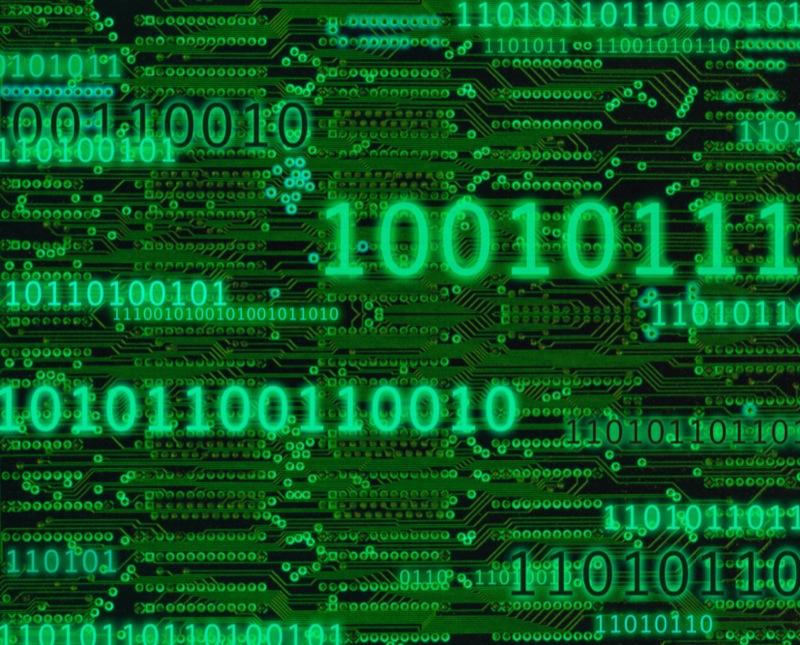
\includegraphics[width=0.382\textwidth]{pictures/binary}
  \end{center}
%\caption{A gull}
\end{wrapfigure}
Es ist nicht genau bekannt, seit wann die Menschen Zahlen benutzen. Die ersten Darstellungen von Zahlen waren wahrscheinlich Striche. Das \"alteste bekannte Beispiel ist ein Knochen eines Wolfes, in dem 55 tiefe Kerben eingeritzt sind. Diese Darstellung wird heute noch gerne auf Bierdeckeln oder f\"ur einfache Z\"ahlaufgaben, beispielsweise beim Jassen, verwendet. Man spricht hier von einem \emph{un\"aren} Zahlensystem, weil alle Zahlen mit nur einem Zeichen (Strich) dargestellt werden. Der \"Ubersicht wegen fasst man h\"aufig f\"unf Striche zusammen, indem der f\"unfte Strich quer \"uber die vier Einzelstriche gelegt wird.
\begin{ueb}
Weshalb fasst man just f\"unf Striche zu einem B\"undel zusammen?
\end{ueb}

\subsubsection{Zahlen in \"Agypten (ca. 3000 v. Chr.)}
Die \"Agypter entwickelten ein eigenes Zahlensystem mit unterschiedlichen Zeichen f\"ur die Zahlen $1, 10, 100, 1000, \dots, 10^6$.
\begin{figure}[h!]
\begin{center}
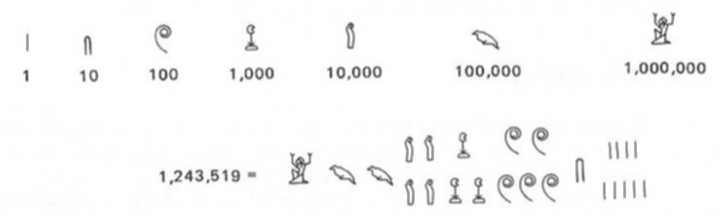
\includegraphics[width=1\textwidth]{pictures/aegyptischeZahlen}
\end{center}
\caption{\"Agyptische Zahlen}
\end{figure}
Dies ist ein sogenanntes \emph{Additionssystem} zur Basis $10$, wobei jede Zehnerpotenz ($10^0, \dots, 10^6$) ein eigenes Zeichen hat und die Zahl die Summe der Werte ihrer Ziffern ist. \"Ubrigens, die \"Agypter waren vermutlich auch die Ersten, welche Zeichen f\"ur Br\"uche einf\"uhrten.

\begin{ueb}[ägyptisch]
\"Ubersetze folgende Zahlen ins \glqq \"Agyptische\grqq:\\

\begin{minipage}{0.4\textwidth}
\begin{enumeratea}
\item $2300654$
\end{enumeratea}
\end{minipage}
\begin{minipage}{0.23\textwidth}
\begin{enumeratea}
\addtocounter{enumi}{1}
\item $44629$
\end{enumeratea}
\end{minipage}
\end{ueb}
\begin{ueb}[mal so mal so]
Finde Zahlen, die in der \"agyptischen Schreibweise mehr Zeichen ben\"otigen als in unserer Schreibweise. Finde auch Zahlen, die bei den \"Agyptern k\"urzer geschrieben wurden.
\end{ueb}
\begin{ueb}[vorteil?]
Beschreibe Vor- und Nachteile der \"agyptischen Zahlenschreibweise ge\-gen\-\"uber unserem heutigen System.
\end{ueb}

\subsubsection{Zahlen in Babylonien (ca. 2000 v. Chr.)}
\begin{figure}[h]
\begin{center}
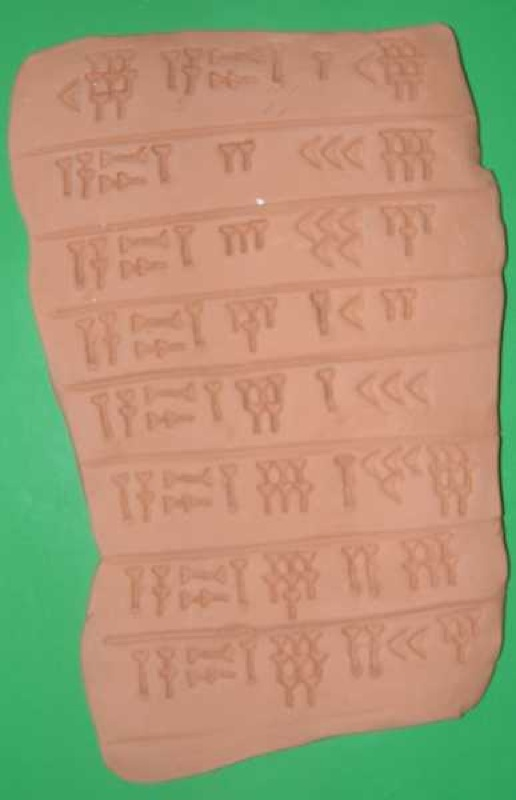
\includegraphics[width=0.35\textwidth]{pictures/babylontafel}\hspace*{0.2cm}
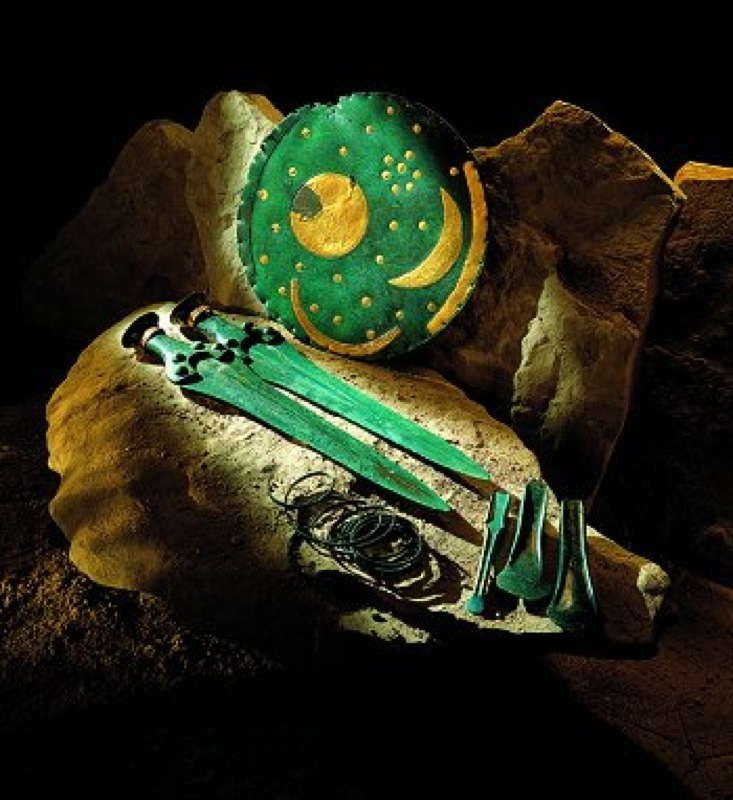
\includegraphics[width=0.35\textwidth]{pictures/babylonuhr}
\end{center}
\caption{Babylonische Rechentafel und Sternkarte}
\end{figure}
Die Babylonier verwendeten als eines der ersten V\"olker ein sogenanntes \emph{Positionssystem}. Der Wert eines Zeichens h\"angt auch von dessen Position ab. W\"ahrend wir heute in unserem Dezimalsystem (Basis 10) die Ziffern $0, 1, 2, \dots, 9$ verwenden, brauchten die Babylonier in ihrem Sechzigersystem $59$ Ziffern. Ein Zeichen f\"ur die Null, das \glqq Nichts\grqq, gab es damals noch nicht.
\begin{ueb}[Zahlzeichen]
Finde eine Darstellung der Zahlzeichen der Babylonier, und schreibe das Wesentliche dieser Darstellung auf, so dass du mit deinen Notizen jede Zahl in Babylonisch schreiben kannst.
\end{ueb}

Abschliessend noch ein Beispiel, wie diese Zeichen verwendet werden.
\begin{center}
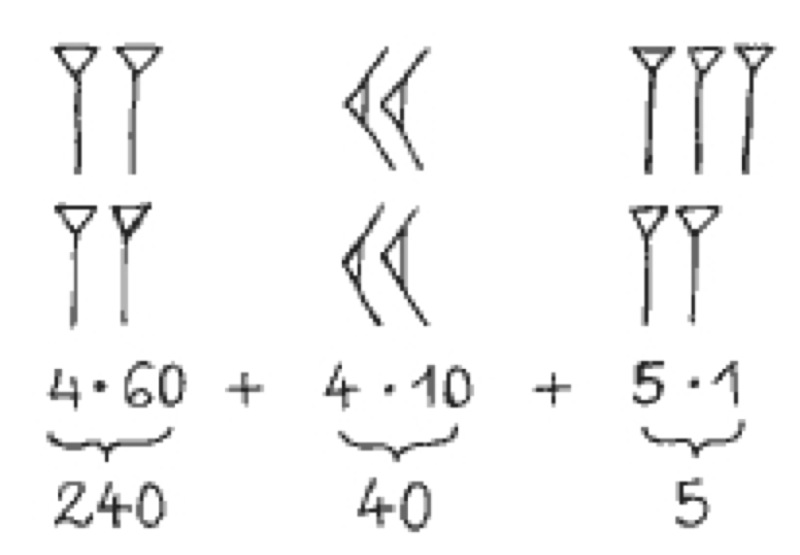
\includegraphics[width=5cm]{pictures/babylon285}
\end{center}
\begin{ueb}[übersetze]
\"Ubersetze folgende Zahlen ins \glqq Babylonische\grqq:

\begin{minipage}{0.4\textwidth}
\begin{enumeratea}
\item $2381$
\end{enumeratea}
\end{minipage}
\begin{minipage}{0.23\textwidth}
\begin{enumeratea}
\addtocounter{enumi}{1}
\item $829$
\end{enumeratea}
\end{minipage}
\end{ueb}

\subsubsection{Zahlen in Indien und Arabien}
Die Ziffern, wie wir sie heute verwenden, haben ihren Ursprung in Indien und Arabien. Sie wurden unter anderem durch Kaufleute wie Fibonacci im 13. Jahrhundert nach Europa gebracht, konnten sich aber erst sp\"ater gegen die r\"omischen Zahlen durchsetzen.

Eine grossartige Leistung des menschlichen Geistes stellt die Erfindung der Zahl Null dar. F\"ur die Menschen war es lange Zeit unvorstellbar, ein Zeichen f\"ur \glqq Nichts\grqq\  zu gebrauchen. Bei Positionssystemen ist ein Zeichen f\"ur Null als Platzhalter aber unentbehrlich. Ohne die Null k\"onnte zum Beispiel $12$ mehrere Bedeutungen haben: $12, 102, 120, 1200, \dots$.
\begin{figure}[h]
\begin{center}
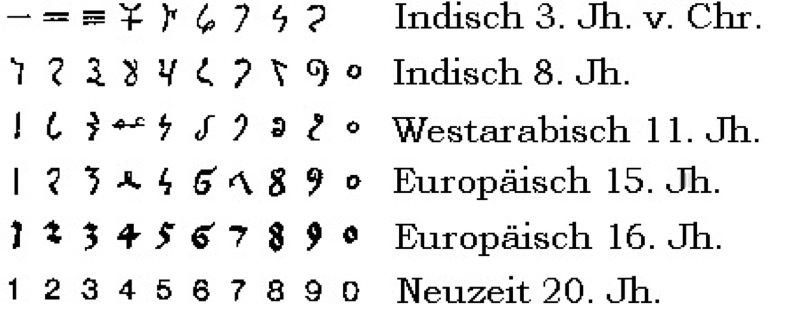
\includegraphics[width=0.7\textwidth]{pictures/entwzahl}
\end{center}
\caption{Evolution von den indischen bis zu den heutigen arabischen Ziffern}
\end{figure}

\begin{ueb}[römisch]
Notiere die r\"omischen Zahlzeichen, und finde Regeln zur Bildung von Zahlen in der r\"omischen Schreibweise.
\end{ueb}
\begin{ueb}[Jahreszahl]
Schreibe $\the\year$ mit r\"omischen Zahlzeichen; und $1848$.
\end{ueb}
\begin{ueb}[magisches Quadrat]
Stelle ein magisches $4\times4$ Quadrat mit r\"omischen Zahlen her.
\end{ueb}

\begin{figure}
\begin{center}
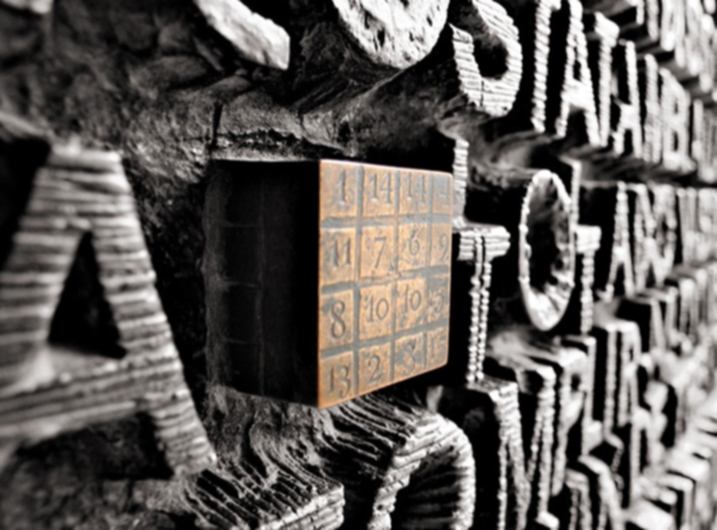
\includegraphics[width=0.618\textwidth]{pictures/magquadr}
\end{center}
\caption{Magisches Quadrat am Tor der Familia Sagrada}
\end{figure}

\subsection{Zahlensysteme}
Ein Zahlensystem wird zur Darstellung von Zahlen verwendet. Eine Zahl wird dabei nach den Regeln des Zahlensystems als Folge von Ziffern dargestellt. Man unterscheidet im Wesentlichen zwischen Additionssystemen und Stellenwertsystemen (Positionssystemen).
\subsection{Additionssysteme}
In einem Additionssystem wird eine Zahl als Summe der Werte ihrer Ziffern dargestellt. Dabei spielt die Position der einzelnen Ziffern keine Rolle.
\begin{ueb}[bsp add]
Nenne zwei Additionssysteme.
\end{ueb}
\subsection{Positionssysteme}
In einem Positionssystem bestimmt die Stelle (Position) den Wert der jeweiligen Ziffer. Die \glqq niederwertigste\grqq\ Position steht dabei im Allgemeinen rechts.

Ein Stellenwertsystem hat eine Basis $b$. Jede Zifferposition hat einen Wert, der einer Potenz der Basis entspricht. F\"ur die $k$-te Position hat man einen Wert von $b^{k-1}$.

Die Berechnung des Zahlenwertes erfolgt durch Multiplikation der einzelnen Ziffern $z_i$ mit den zugeh\"origen Stellenwerten $b_i$ und Summation dieser Produkte:
$$\text{Zahlenwert} = z_n\cdot b^n+\dots+z_i\cdot b^i+\dots+z_0\cdot b^0.$$
\begin{bsp}
Unter
\marginnote{
\qrcode{
https://www.youtube.com/watch?v=j3uGEq0mXIk}
}
der Zahl $1257$ im \"ublichen Dezimalsystem (d.h. die Basis ist $10$) verstehen wir den Wert
$$1\cdot10^3+2\cdot10^2+5\cdot10^1+7\cdot10^0 = 1257.$$
\end{bsp}
\begin{ueb}[bsp pos]
Nenne ein Positionssystem ausser das Dezimalsystem.
\end{ueb}
Bei einigen Naturv\"olkern sind auch noch Zahlensysteme zu anderen Basen gefunden worden. Vergleichsweise weit verbreitet ist das System zur Basis 20. Bei diesen V\"olkern werden in der Regel zum Z\"ahlen neben den Fingern auch noch die F\"usse verwendet.

Mit der Beschr\"ankung des niedrigsten Exponenten auf $0$ kann man nur ganze Zahlen darstellen. L\"asst man auch negative Exponenten zu, kann man auch rationale Zahlen in einem Stellenwertsystem schreiben, wobei der \"Ubergang vom nichtnegativen zum negativen Exponenten durch ein Trennzeichen markiert wird, beispielsweise ein Komma:
$$1\cdot10^2+2\cdot10^1+1\cdot10^0+4\cdot10^{-1}+7\cdot10^{-2}=121,47$$

\begin{ueb}[binär]
Die Idee des Positionssystems mit einer bestimmten Basis wird auch beim Bin\"arsystem (Basis $2$) verwendet. Computer stellen Zahlen nur mit den Ziffern $0$ und $1$ dar und zwar als magnetische Polung oder elektrisches Signal (Nord oder S\"ud bzw. Plus oder Minus).
Die bin\"are Zahl $1011$ entspricht der Dezimalzahl
$$1\cdot2^3+0\cdot2^2+1\cdot2^1+1\cdot2^0=8+2+1=11.$$
Stelle die Dezimalzahlen von $1$ bis $20$ im Bin\"arsystem dar. Beschreibe dein Vorgehen.
\end{ueb}
\begin{ueb}[bin dec]
Verwandle folgende Bin\"arzahlen in Dezimalzahlen
$$1\qq11\qq111\qq1111\qq\dots$$
und
$$10\qq100\qq1000\qq10000\qq\dots$$
\end{ueb}
\begin{ueb}[dec bin]
Finde f\"ur die Dezimalzahlen $34$ und $37$ die Bin\"arschreibweise.
\end{ueb}

\subsection{Das Sexagesimalsystem}

Von den Kulturv\"olkern ist mir nur von den Sumerern und Babyloniern bekannt, dass sie ein Stellenwertsystem benutzten. Das Wissen um den Vorteil eines Stellenwertsystems ging danach wieder verloren, so dass weder die Griechen noch die R\"omer ein solches Zahlensystem verwendeten. In diesem Kontext sei erneut auf die praktischen Vorteile eines Stellenwertsystems hingewiesen, zum Beispiel im kaufm\"annischen Bereich. Die Verachtung der Griechen f\"ur eine anwendungsorientierte Mathematik mag erkl\"aren, warum dieses so erfindungsreiche Volk keine Anstalten machte, sein kompliziertes, alphabetisches System durch ein Stellenwertsystem zu ersetzen. Im Folgenden wollen wir auf das babylonische Zahlensystem eingehen, da es bis heute in unserem Alltag pr\"asent ist.

Das babylonische Zahlensystem ist ein Stellenwertsystem zur Basis 60, mit dem beliebig grosse, aber auch beliebig kleine Zahlen systematisch dargestellt werden k\"onnen. Die Babylonier benutzten eine Keilschrift, die durch das Eindr\"ucken von Griffeln in Tontafeln entstand. Hier die ersten 59 Zahlen.
\begin{figure}[h]
\begin{center}
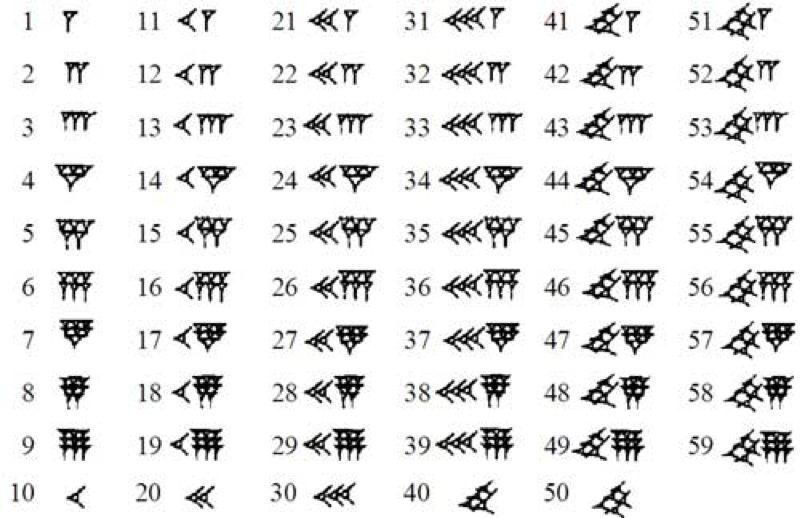
\includegraphics[width=0.7\textwidth]{pictures/babylonzahlen}
\end{center}
\caption{Babylonische Zahlen von 1 bis 59}
\end{figure}
Jede dieser oben aufgef\"uhrten Zahlen ist als eine Ziffer zu interpretieren. Erst bei Zahlen \"uber $59$ wird naturgem\"ass die n\"achste Stelle benutzt. Sie wird, wie auch bei unserem Dezimalsystem, nach links einger\"uckt.
\begin{center}
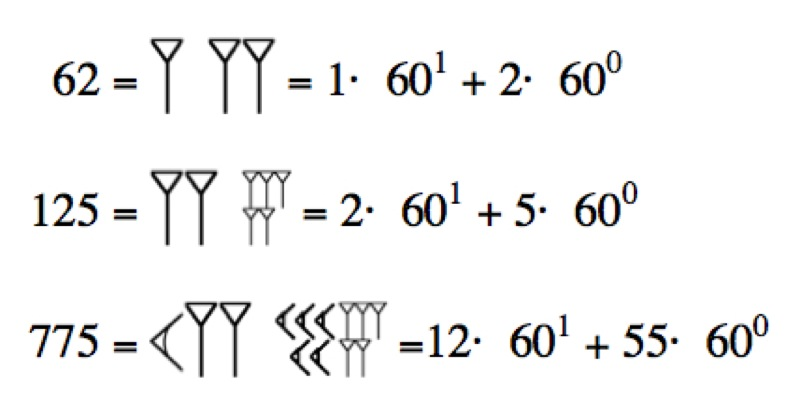
\includegraphics[width=0.5\textwidth]{pictures/babylongrossezahlen}
\end{center}
Genauso interessant ist, dass die Babylonier ihr Stellenwertsystem auch f\"ur Nachkommazahlen nutzten. Dabei kam ihnen die vielf\"altige Teilbarkeit der Zahl 60 zugute --- dies war vermutlich auch der Grund, weshalb das Sexagesimalsystem \"uberhaupt eingef\"uhrt wurde. Ein Zeichen f\"ur das \glqq Komma\grqq\ war nicht vorhanden, so dass die Zuordnung der Stellen zu den $60$-er Potenzen nicht eindeutig war. Welche Position z.B. die $60^0$-Stelle hat, musste aus dem Kontext erraten werden.
\begin{center}
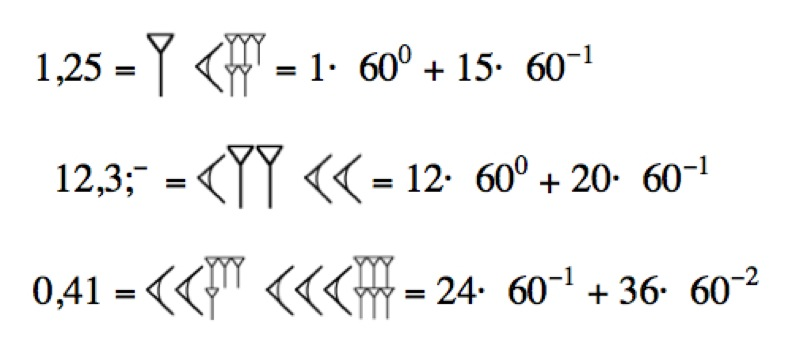
\includegraphics[width=0.4\textwidth]{pictures/babylonnachkomma}
\end{center}

\begin{figure}
\begin{center}
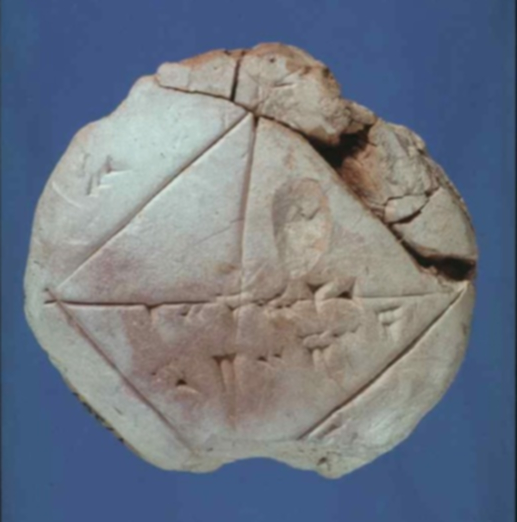
\includegraphics[width=0.45\textwidth]{pictures/tontafel}
\end{center}
\caption{Babylonische Tontafel, 7289 v.Chr.}\label{abb:tontafel}
\end{figure}

Eine genaue Untersuchung des Objekts aus Abbildung \ref{abb:tontafel} auf Seite \pageref{abb:tontafel} f\"ordert folgendes Schriftbild zu Tage, das in Abbildung \ref{interpretation} auf Seite \pageref{interpretation} deutlicher zu erkennen ist.

Es zeigt sich, dass man ein sinnvolles Ergebnis kriegt, wenn man die erste \glqq1\grqq\ mit $1\cdot60^0$ identifiziert. Wir erhalten so f\"ur die erste Zeile
$$1\cdot60^0+24\cdot60^{-1}+51\cdot60^{-2}+10\cdot60^{-3}$$
\begin{ueb}[irrational]
Welche Zahl wird hier vermutlich beschrieben?
\end{ueb}

\begin{figure}
\begin{center}
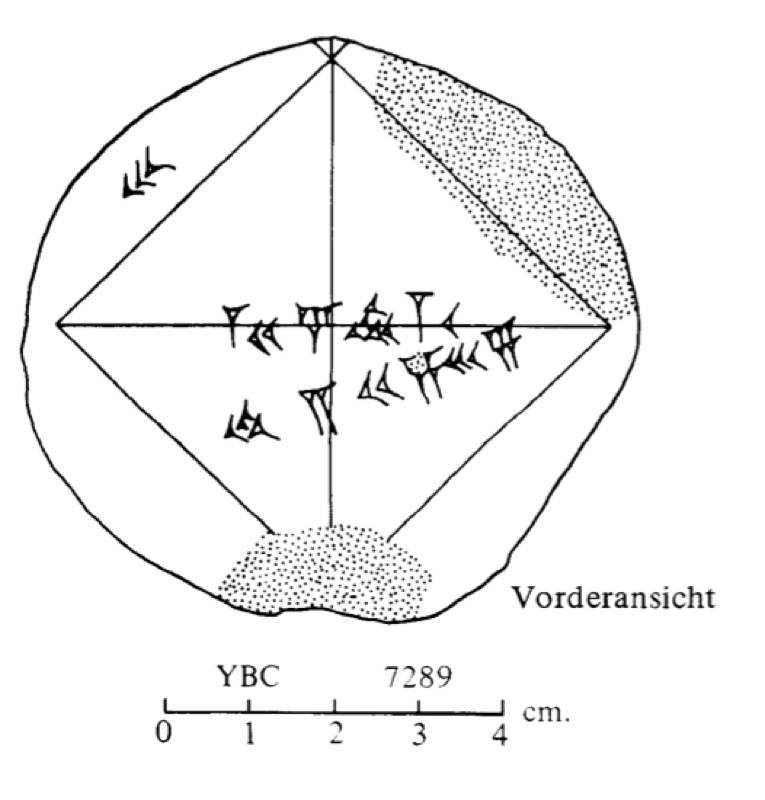
\includegraphics[width=0.35\textwidth]{pictures/tontafelschema}
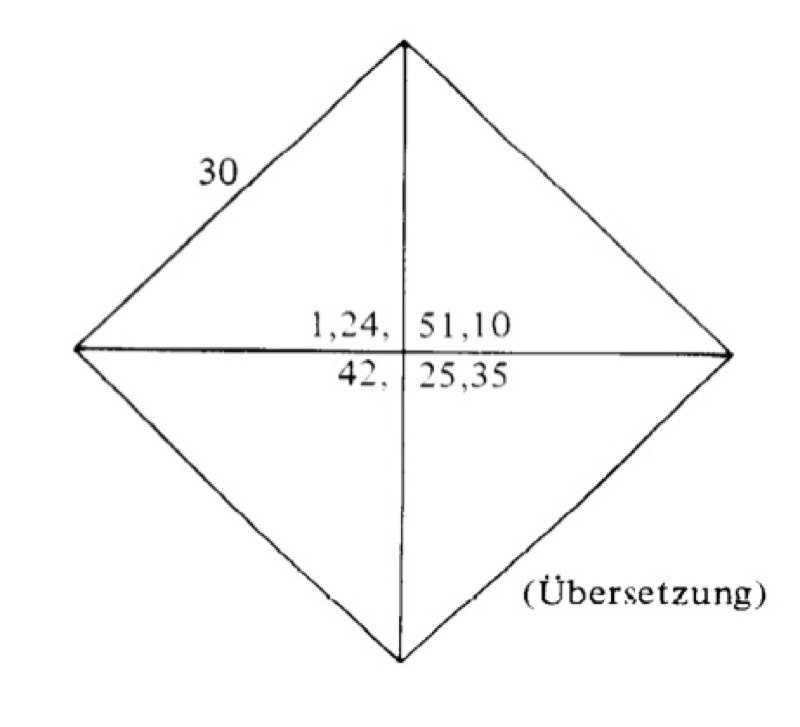
\includegraphics[width=0.35\textwidth]{pictures/schema}
\end{center}
\caption{Schema und \"Ubersetzung der Zahlen}\label{interpretation}
\end{figure}

\begin{landscape}
\begin{figure}[h]
\begin{center}
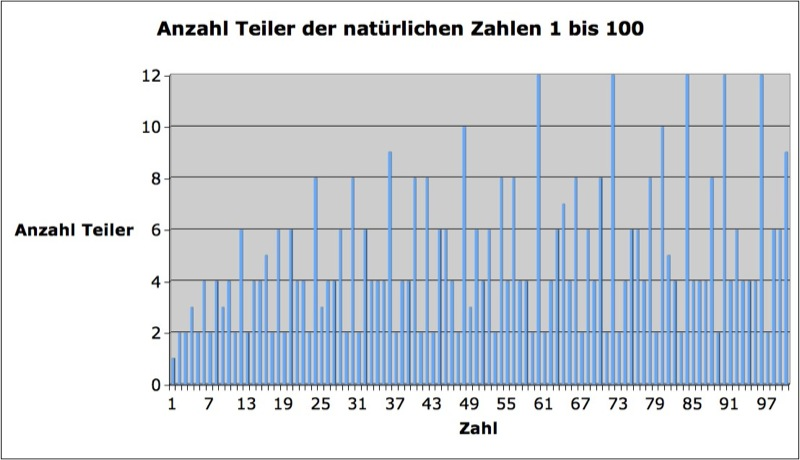
\includegraphics[height=0.7\textheight]{pictures/anzahlteiler}
\end{center}
\caption{Anzahl Teiler der ersten hundert nat\"urlichen Zahlen}
\end{figure}
\end{landscape}

\clearpage

\appendix

\section{Das Bin\"arsystem}

Wie k\"onnte eine Codierung von Zeichen im Computer realisiert werden? Der Computer arbeitet mit elektrischem Strom. Das heisst er kann lediglich die beiden Zust\"ande \glqq Strom an\grqq\ und \glqq Strom aus\grqq\ unterscheiden. Man codiert $1$ f\"ur den ersten und $0$ f\"ur den zweiten Zustand. Die Information, die durch den Strom in einer Leitung codiert ist, heisst \emph{ein Bit} (binary digit). So lassen sich bloss zwei Zeichen codieren. Kombiniert man aber zwei Leitungen, lassen sich nun vier Zust\"ande unterscheiden:
\begin{center}
\begin{tabular}{c|c}
Leitung 1 & Leitung 2\\ \hline
0 & 0\\
0 & 1\\
1 & 0\\
1 & 1\\
\end{tabular}
\begin{ueb}
Stelle eine Tabelle f\"ur drei Leitungen auf.
\end{ueb}
\end{center}
Dies reicht nat\"urlich f\"ur unsere Zwecke noch nicht.
\begin{frage}
Wie viele Leitungen braucht man, um alle Buchstaben des Alphabets codieren zu k\"onnen?
\end{frage}
In der Informatik ist es \"ublich, acht Leitungen zur Speicherung von Informationen zusammenzufassen. Insgesamt lassen sich damit $2^8=256$ verschiedene Zeichen darstellen. Man spricht bei dieser B\"undelung von acht Leitungen vom Informationsgehalt ein \emph{Byte}.
\begin{bem}
Fr\"uher rechnete man noch in Kilobyte, was ca. 1000 Bytes entspricht. Kilo wurde in diesem Zusammenhang nicht wie \"ublich f\"ur den Wert Tausend verwendet, sondern f\"ur $2^{10}=1024\approx1000$. Deshalb ist zum Beispiel ein Megabyte = 1024 Kilobyte.
\end{bem}
Nun zur n\"achsten Frage: Wie rechnet der Computer mit diesen Bin\"arzahlen? Dabei gehen wir hier aber nicht auf die Frage ein, wie diese Rechnungen technisch realisiert werden, sondern betrachten nur die algebraischen Aspekte des Rechnens mit Bin\"arzahlen.

Die Addition von Bin\"arzahlen funktioniert prinzipiell genau so, wie die Addition von Dezimalzahlen.
\begin{ueb}
Addiere schriftlich die Bin\"arzahlen $1001011$ und $101011$.
\end{ueb}
\noindent Werden mehrere Bin\"arzahlen addiert, kann der \"Ubertrag nat\"urlich auch gr\"osser als $1$ werden.
\begin{ueb}
Addiere schriftlich die Bin\"arzahlen $1001011$, $101011$ und $101011$.
\end{ueb}
\begin{ueb}
Berechne folgende Aufgaben, indem du alle Summanden ins Bin\"arsystem \"uberf\"uhrst, darin addierst und das Ergebnis schliesslich ins Dezimalsystem zur\"uck \"uber\-setzt. Kontrolliere mit der dezimalen Rechnung.
\begin{enumeratea}
\item $35+17$
\item $119+31$
\item $63+63+1$
\end{enumeratea}
\end{ueb}



\cleardoublepage
\listoffigures
%\listoftables
%\newpage
%\nocite{*}
%\bibliographystyle{plain}
%\bibliography{preamble/literaturgoogle}
\end{document}